%%%%%%%%%%%%%%%%%%%% author.tex %%%%%%%%%%%%%%%%%%%%%%%%%%%%%%%%%%%
%
% sample root file for your "contribution" to a contributed volume
%
% Use this file as a template for your own input.
%
%%%%%%%%%%%%%%%% Springer %%%%%%%%%%%%%%%%%%%%%%%%%%%%%%%%%%


% RECOMMENDED %%%%%%%%%%%%%%%%%%%%%%%%%%%%%%%%%%%%%%%%%%%%%%%%%%%
\documentclass[graybox]{svmult}

% choose options for [] as required from the list
% in the Reference Guide

\usepackage{amsmath}
\usepackage{amssymb}
\usepackage{mathptmx}       % selects Times Roman as basic font
\usepackage{helvet}         % selects Helvetica as sans-serif font
\usepackage{courier}        % selects Courier as typewriter font
\usepackage{type1cm}        % activate if the above 3 fonts are
                            % not available on your system
%
\usepackage{makeidx}         % allows index generation
\usepackage{graphicx}        % standard LaTeX graphics tool
                             % when including figure files
\usepackage{multicol}        % used for the two-column index
\usepackage[bottom]{footmisc}% places footnotes at page bottom


%%%%%%%%%%%%%%%%%%%%

\newcommand{\Hess}{\operatorname{Hess}}



\usepackage{tikz}
\usetikzlibrary{decorations.markings}
\usetikzlibrary{decorations.pathmorphing}
\usetikzlibrary{arrows, snakes}
\usetikzlibrary{shapes.geometric, calc,decorations.pathreplacing}
\usetikzlibrary{backgrounds}
\usetikzlibrary{fit}
\usepackage{caption}
%%%%%%%%%%%%%%%%%%%%

% see the list of further useful packages
% in the Reference Guide

\makeindex             % used for the subject index
                       % please use the style svind.ist with
                       % your makeindex program
                       
                       
                       

%%%%%%%%%%%%%%%%%%%%%%%%%%%%%%%%%%%%%%%%%%%%%%%%%%%%%%%%%%%%%%%%%%%%%%%%%%%%%%%%%%%%%%%%%

\begin{document}

\title*{Information geometry in portfolio theory}
% Use \titlerunning{Short Title} for an abbreviated version of
% your contribution title if the original one is too long
\author{Ting-Kam Leonard Wong}
\authorrunning{T.-K.~L. Wong}
% Use \authorrunning{Short Title} for an abbreviated version of
% your contribution title if the original one is too long
\institute{Ting-Kam Leonard Wong \at University of Toronto, \email{tkleonardwong@gmail.com}}
%
% Use the package "url.sty" to avoid
% problems with special characters
% used in your e-mail or web address
%
\maketitle

%\abstract*{}
%\abstract{}


\section{Introduction}
In the first chapter of their influential monograph \cite[p.1]{AN02} Amari and Nagaoka explained the key idea of information geometry as follows:
\begin{quote}
Information geometry ... allow[s] us to take problems from a variety of fields: statistics, information theory, and control theory; visualize them geometrically; and from this develop novel tools with which to extend and advance these fields.
\end{quote}
In this chapter we show that this principle can be fruitfully applied to financial problems. We review some recent development in the field of stochastic portfolio theory (SPT) motivated by information geometry, present illustrative examples and an extension of functional portfolio generation (announced in \cite{W17a} which is an early version of this paper), and suggest several problems for further study. It is hoped that the materials will be of interest to researchers in both information geometry and mathematical finance. The topics discussed are heavily influenced by the author's research interests. Other financial applications of information geometry are briefly reviewed in Section \ref{sec:literature}.

\subsection{Main ideas: market diversity and volatility} \label{sec:main.idea}
To set the stage let us consider a universe of stocks represented by a capitalization-weighted index. A typical example is the S\&P 500 Index which includes a significant portion of the US stock market. In a capitalization-weighted index, the influence of a stock is proportional to its market capitalization. Following the standard set up of stochastic portfolio theory (see for example \cite{F02, FK09}), if we let $X_i(t) > 0$ be the market capitalization of stock $i$ at time $t$, then
\begin{equation} \label{eqn:market.weight}
\mu_i(t) := \frac{X_i(t)}{X_1(t) + \cdots + X_n(t)}
\end{equation}
is the {\it market weight} of the stock. Throughout this chapter we let time be discrete. Let $n \geq 2$ be the number of stocks in the market. The vector $\mu(t) = (\mu_1(t), \ldots, \mu_n(t))$ takes values in the open unit simplex $\Delta_n$ given by
\begin{equation*}
\begin{split}
\Delta_n &:= \{p = (p_1, \ldots, p_n) \in (0, 1)^n: p_1 + \cdots + p_n = 1\}.
\end{split}
\end{equation*}
Its closure in $\mathbb{R}^n$ is denoted by $\overline{\Delta}_n$.  The vector $\mu(t)$ may also be regarded as the portfolio weights of the {\it market portfolio}. 

A major objective of SPT is to construct investment strategies that beat the market under  realistic conditions on market behaviors. These portfolios are called {\it relative arbitrages} with respect to the market portfolio. For more details about this important problem see for example \cite{F02, FK09, FKR17} and their references. As a simple example, Figure \ref{fig:simplex} plots the path of $\{\mu(t)\}$ for a hypothetical $3$-stock market consisting of the US stocks Ford, IBM and Walmart. It should not be surprising that the relative performance of portfolios with respect to the market can be analyzed using appropriate geometries on the simplex.\footnote{In practice the number of stocks changes with time, and the market capitalization may fluctuate due to public offerings and other events. For simplicity these complications are neglected here.}


\begin{figure}[t!]
\centering
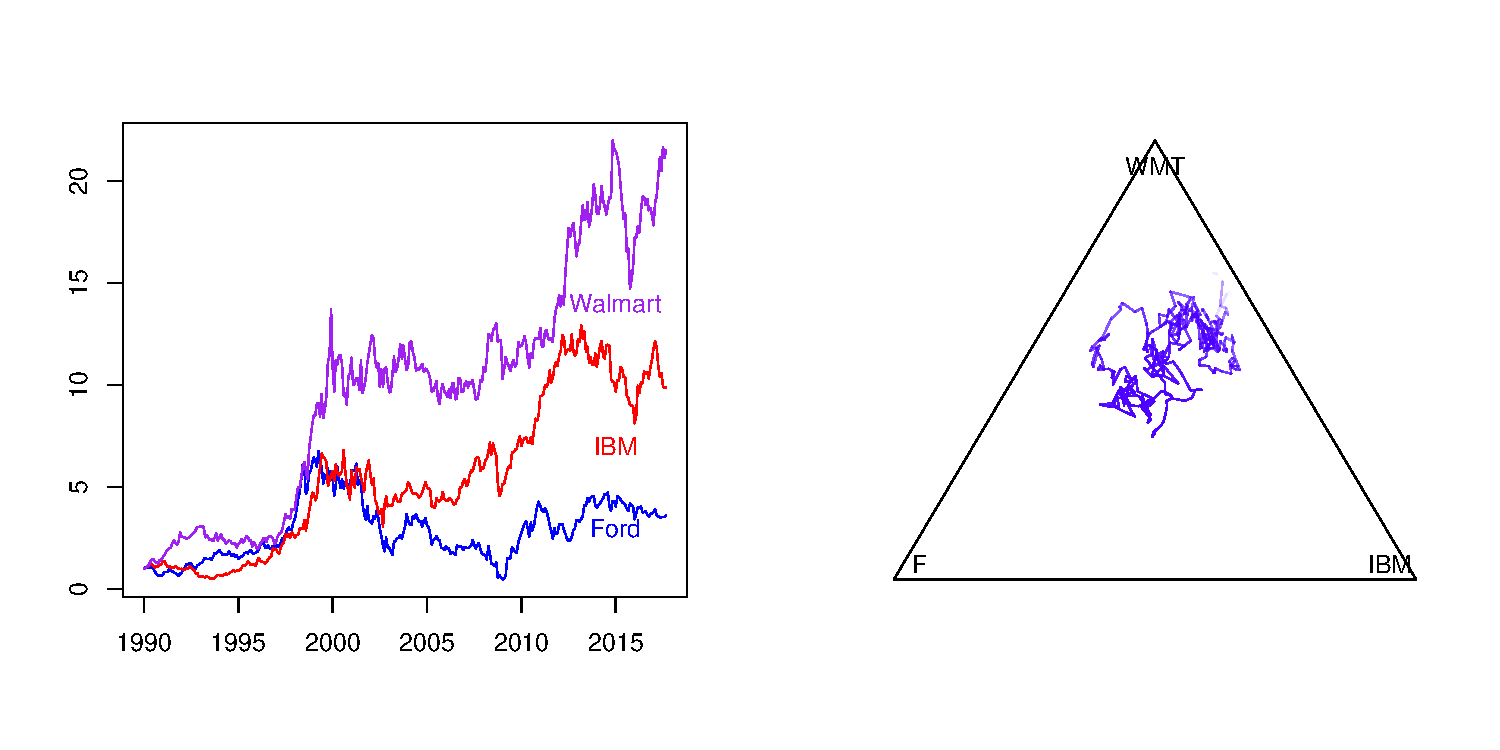
\includegraphics[scale=0.42]{simplex.pdf}
\caption{Left: Monthly prices of the stocks (regarded as the capitalization and normalized to be $1$ from January 1990). Right: Path of the market weight vector $\mu(t)$ in the simplex $\Delta_3$.} \label{fig:simplex}
\end{figure}

Regarding the market as a process in the simplex $\Delta_n$, there are two natural quantities an investor may want to keep track of: {\it diversity} and {\it volatility}. Diversity refers to the degree of capital concentration in the equity market. For example, in Figure \ref{fig:simplex}, the market moves towards the vertex representing Walmart and thus becomes more concentrated. According to \cite{FGH98}, many mutual funds tend to overweight small stocks and underweight large stocks (relative to the market index), so the change in market diversity is a significant predictor of their relative performance. To quantify diversity one introduces a positive {\it concave} function $\Phi: \Delta_n \rightarrow (0, \infty)$, and we say that the market is more diverse when $\Phi(\mu(t))$ is large. Typical examples include the Shannon entropy
\[
\Phi(p) = - \sum_{j = 1}^n p_j \log p_j
\]
as well as the $\lambda$-diversity function
\begin{equation} \label{eqn:diversity}
\Phi(p) = \left( \sum_{j = 1}^n (p_j)^{\lambda} \right)^{1/\lambda},
\end{equation}
where $0 < \lambda < 1$ is a parameter. More examples of measures of diversity can be found in \cite[Chapter 3]{F02}. Note that we allow $\Phi$ to be asymmetric, so it can attain its maximum value at a point other than the barycenter $\overline{e} := \left(\frac{1}{n}, \ldots, \frac{1}{n}\right)$. As it turns out, it is mathematically more convenient to consider its logarithm $\varphi := \log \Phi$. Since $e^{\varphi} = \Phi$ is concave, we say that $\varphi$ is {\it exponentially concave}. We remark that $\varphi$, being the logarithm of a concave function, is itself a concave function. Given $\varphi$, the time series of $\{\varphi(\mu(t))\}$ is an indicator of market diversity (see Figure \ref{fig:decomp} (left)).

\begin{figure*}[t!]
\centering
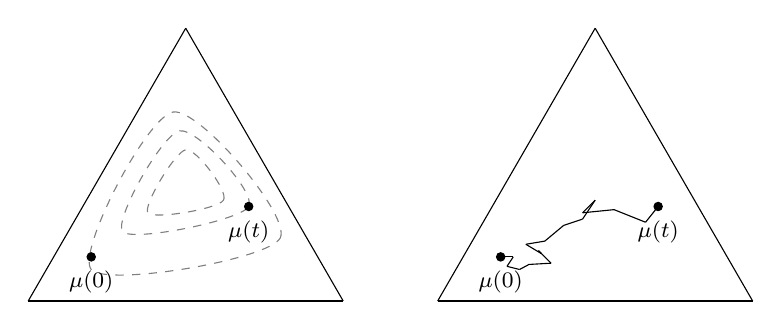
\begin{tikzpicture}[scale = 0.8]
%draw simplex 1
\draw (0, 0) to (5, 0);
\draw (5, 0) to (2.5, 4.33);
\draw (2.5, 4.33) to (0, 0);

\draw [gray, dashed] plot [smooth cycle] coordinates {(1, 0.5) (4,1) (2.3, 3)};
\draw [gray, dashed] plot [smooth cycle] coordinates {(1.5, 1.1) (3.5, 1.5) (2.4, 2.7)};
\draw [gray, dashed] plot [smooth cycle] coordinates {(1.9, 1.4) (3.1, 1.6) (2.5, 2.4)};

\node[circle, draw=black, fill = black, inner sep=0pt, minimum size=3pt, label = below: {\footnotesize $\mu(0)$}] at (1, 0.7)  {};
\node[circle, draw=black, fill = black, inner sep=0pt, minimum size=3pt, label = below: {\footnotesize $\mu(t)$}] at (3.5, 1.5) {};

%draw simplex 2
\draw (6.5, 0) to (11.5, 0);
\draw (11.5, 0) to (9, 4.33);
\draw (9, 4.33) to (6.5, 0);
\node[circle, draw=black, fill = black, inner sep=0pt, minimum size=3pt, label = below: {\footnotesize $\mu(0)$}] at (7.5, 0.7)  {};
\node[circle, draw=black, fill = black, inner sep=0pt, minimum size=3pt, label = below: {\footnotesize $\mu(t)$}] at (10, 1.5) {};

\draw (7.5, 0.7) to (7.7, 0.7);
\draw (7.7, 0.7) to (7.6, 0.55);
\draw (7.6, 0.55) to (7.8, 0.5);
\draw (7.8, 0.5) to (7.95, 0.58);
\draw (7.95, 0.58) to (8.3, 0.6);
\draw (8.3, 0.6) to (8.1, 0.8);
\draw (8.1, 0.8) to (8.15, 0.75);
\draw (8.15, 0.75) to (7.9, 0.9);
\draw (7.9, 0.9) to (8.2, 0.95);
\draw (8.2, 0.95) to (8.5, 1.2);
\draw (8.5, 1.2) to (8.8, 1.3);
\draw (8.8, 1.3) to (9, 1.6);
\draw (9, 1.6) to (8.8, 1.4);
\draw (8.8, 1.4) to (9.3, 1.45);
\draw (9.3, 1.45) to (9.8, 1.25);
\draw (9.8, 1.25) to (10, 1.5);


%\node [black, left] at (0, 5) {{\footnotesize $c_1$}};
%\node [black, right] at (10, 2) {{\footnotesize $c_2$}};
%\node [black, right] at (5, 5.1) {{\footnotesize $c_n$}};
%\node [black, right] at (4.7, 0.06) {{\footnotesize $\Delta_n$}};

\end{tikzpicture}
\captionsetup{labelformat=empty}

\caption{Left: Change in market diversity measured by $\varphi$. The dashed curves represent level sets of $\varphi$. Right: Market volatility can be measured by the $L$-divergence ${\bf D} \left[\cdot \mid \cdot\right]$.}
\label{fig:decomp}
\end{figure*}

The volatility of the market weight $\mu(t)$ refers to the volatility of the stocks {\it relative to each other}. Anticipating the use of information geometry, note that the Euclidean quadratic variation (in discrete time) given by
\begin{equation} \label{eqn:quadratic variation}
\sum_{s = 0}^{t - 1} | \mu(s + 1) - \mu(s) |^2
\end{equation}
may not be appropriate because the Euclidean norm on the simplex may not have a financial meaning (see however Example \ref{eg:quadratic}). In particular, the same displacement $v = \mu(s + 1) - \mu(s)$ (approximated by a tangent vector) should have different norms on different portions of the simplex. Depending on the application, market volatility along a path should be quantified by a sum like
\[
\sum_{s = 0}^{t - 1} {\bf D}\left[ \mu(s + 1) \mid \mu(s) \right],
\]
where ${\bf D}\left[ \cdot \mid \cdot \right]: \Delta_n \times \Delta_n \rightarrow [0, \infty)$ is possibly asymmetric in its arguments. In information geometry we say that ${\bf D}\left[ \cdot \mid \cdot \right]$ a {\it divergence} (a rigorous definition is given in Definition \ref{def:divergence}). Intuitively, the asymmetry of ${\bf D}\left[ \cdot \mid \cdot \right]$ reflects the effect of time: the time-reversed path $\tilde{\mu}(t) = \mu(T - t)$ probably have different impacts on the portfolio. %We will see that this asymmetric vanishes in the continuous time limit, but the metric generally depends on the position in the simplex.

The main idea of this chapter is the following. A differentiable, exponentially concave function $\varphi: \Delta_n \rightarrow \mathbb{R}$ defines an {\it $L$-divergence} ($L$ stands for logarithmic)
\begin{equation} \label{eqn:L.divergence}
{\bf D}^{(1)}\left[q \mid p \right] := \log \left(1 + \nabla \varphi(p) \cdot (q - p)\right) - \left( \varphi(q) - \varphi(p) \right) \geq 0, \quad p, q \in \Delta_n,
\end{equation}
which can be used to quantify market volatility. (The superscript will become clear in Definition \ref{def:L.alpha.divergence}.) An important example of $L$-divergence is the {\it excess growth rate} (also known as the {\it diversification return} \cite{BF92}) defined for a fixed portfolio vector $\pi \in \overline{\Delta}_n$ by
\begin{equation} \label{eqn:excess.growth}
{\bf T}_{\pi} \left[q \mid p\right] := \log \left( \sum_{i = 1}^n \pi_i \frac{q_i}{p_i} \right) - \sum_{i = 1}^n \pi_i \log \frac{q_i}{p_i}.
\end{equation}
The corresponding exponentially concave function is $\varphi(p) = \sum_{i = 1}^n \pi_i \log p_i$. Note that the $L$-divergence is different from the classical Bregman divergence of a concave function:
\begin{equation}  \label{eqn:Bregman.divergence}
{\bf D}^{(0)}\left[q \mid p\right] := \nabla \varphi(p) \cdot (q - p) - \left( \varphi(q) - \varphi(p) \right).
\end{equation}
The most important example of Bregman divergence is the relative entropy
\begin{equation} \label{eqn:relative.entropy}
{\bf H} \left(q \mid p\right) := \sum_{i = 1}^n q_i \log \frac{q_i}{p_i},
\end{equation}
where the potential function $\varphi$ is the Shannon entropy. Comparing \eqref{eqn:excess.growth} and \eqref{eqn:relative.entropy}, we see that the excess growth rate involves a nonlinear transformation of an integral, whereas the relative entropy is itself an integral. In Example \ref{eg:diversity} we show that the R\'{e}nyi entropy generates the R\'{e}nyi divergence in the sense of $L$-divergence and is related to the diversity function \eqref{eqn:diversity}.

In Section \ref{sec:fgp}, we will show that the $L$-divergence determines uniquely an investment strategy, called a {\it multiplicatively generated portfolio}, whose performance $V(t)$ relative to the market has the pathwise decomposition
\begin{equation} \label{eqn:fgp.decomp}
\log V(t) - \log V(0) = \varphi(\mu(t)) - \varphi(\mu(0)) + \sum_{s = 0}^{t - 1} {\bf D}^{(1)}\left[\mu(s + 1) \mid \mu(s)\right]. 
\end{equation}
From this decomposition, as long as $\varphi(\mu(t))$ remains bounded and the cumulative volatility grows at a steady rate, the portfolio will outperform the market in the long run (see Proposition \ref{prop:relative.arbitrage}). Furthermore, the dualistic geometry induced by the $L$-divergence (in the sense of \cite{E83, E92}; also see \cite{A16}) has interesting financial applications (see Section \ref{sec:pyth}). In a continuous time framework and without using geometric concepts, these portfolios were first introduced by Fernholz \cite{F99, F02}. Here we adopt the discrete time, geometric approach established in \cite{PW15, PW16}.

Following \cite{W17a, W17b}, in Section \ref{sec:general.portfolio} we will generalize the portfolio construction using the $L^{(\alpha)}$-divergence:

\begin{definition}[$L^{(\alpha)}$-divergence] \label{def:L.alpha.divergence}
Let $\varphi: \Delta_n \rightarrow \infty$ be differentiable and $\alpha$-exponentially concave, i.e, $e^{\alpha \varphi}$ is concave. The $L^{(\alpha)}$-divergence of $\varphi$ is defined for $p, q \in \Delta_n$ by
\begin{equation} \label{eqn:L.alpha.divergence}
{\bf D}^{(\alpha)}\left[q \mid p \right] := \frac{1}{\alpha}\log \left(1 + \alpha \nabla \varphi(p) \cdot (q - p)\right) - \left( \varphi(q) - \varphi(p) \right),
\end{equation}
\end{definition}

Our framework covers also the {\it additively generated portfolio} introduced recently in \cite{KR17}. Note that the $L$-divergence is the $L^{(1)}$-divergence, and the Bregman divergence is equal to ${\bf D}^{(\alpha)}$ as $\alpha \downarrow 0$, so we will also call it the $L^{(0)}$-divergence. Using obvious notations, we have the identity
\begin{equation} \label{eqn:L.alpha.divergence.identity}
{\bf D}^{(\alpha)}_{\varphi} \left[ \cdot \mid \cdot \right] \equiv \frac{1}{\alpha} {\bf D}^{(1)}_{\alpha \varphi} \left[ \cdot \mid \cdot \right].
\end{equation}
According to the results obtained recently in \cite{W17b}, it appears that the $L^{(\alpha)}$-divergence is the canonical interpolation between the Bregman divergence and the $L$-divergence, and plays a fundamental role in information geometry.

\subsection{Financial applications of information geometry} \label{sec:literature}
Instead of conducting an extensive literature review, we content with giving a sample of other financial applications of information geometry. There are mainly two (overlapping) directions: (i) geometries on the state space of financial dynamics, and (ii) optimization using information-geometric quantities such as entropy and divergence. 

Regarding the first direction, the paper \cite{BH01} identifies a yield curve with a distribution function and studies its corresponding dynamics using the Fisher information metric. In option pricing, \cite{T13} applies Tsallis's deformed exponentials and generalized the Black-Scholes model to fat-tailed distributions. Though not directly related to finance, the paper \cite{P17} generalizes the concept of multiplicatively generated portfolio map (see Section \ref{sec:fgp}) to a large class of optimal transport problems. The recent work \cite{KY16} applies the Fisher metric in the study of systemic risk.

On the other hand, divergences are frequently useful as objective/cost functionals. In \cite{NMBN11, NMBN13}, the authors generalize Markowitz's mean-variance model to a mean-divergence model, and show that the resulting portfolios have superior performance. Optimization of probabilistic functionals under a divergence constraint is studied \cite{BC13} and applied to model risk.


\subsection{Outline of the paper}
In Section \ref{sec:market.model} we present the market model and introduce two ways of representing a trading strategy and the associated value process. Section \ref{sec:fgp} reviews known results about multiplicatively generated portfolios with an emphasis on ideas and clarity. Motivated by these results and the recently introduced additively generated portfolio, in Section \ref{sec:general.portfolio} we introduce a general framework for functional portfolio generation, where the $L^{(\alpha)}$-divergence arises naturally. Further properties of the $L$-divergence are discussed in Section \ref{sec:futher} and several related problems are stated.

\section{The market model} \label{sec:market.model}
We work under the discrete time, pathwise setting used in our previous papers \cite{PW13, W15, PW15}. Let $n \geq 2$, the number of stocks in the market, be fixed. The data of our model is a sequence $\{\mu(t) = (\mu_1(t), \ldots, \mu_n(t))\}_{t = 0}^{\infty}$ with values in the open unit simplex $\Delta_n$. We regard $\mu(t)$ as the vector of market weights at time $t$. At this point we do not impose any condition on the sequence $\{\mu(t)\}_{t = 0}^{\infty}$. In Proposition \ref{prop:relative.arbitrage} we will give examples of path properties that lead to relative arbitrages. %Extension to continuous time is discussed briefly in Section \ref{sec:continuous.time}.

We consider self-financing trading strategies in this market model. Let us express a strategy in terms of the number of shares held at each point in time. Furthermore, we use the market portfolio as the num\'{e}raire (i.e., unit of price). This means that the (relative) value of stock $i$ is simply the market weight $\mu_i(t)$. We assume that trading is frictionless.

\begin{definition}[Self-financed trading strategy] \label{def:strategy}
A self-financing trading strategy is a sequence $\eta = \{\eta(t)\}_{t = 0}^{\infty}$, with values in $\mathbb{R}^n$, such that the self-financing identity
\begin{equation} \label{eqn:self.financed}
\sum_{i = 1}^n \eta_i(t) \mu_i(t + 1) \equiv \sum_{i = 1}^n \eta_i(t + 1) \mu_i(t + 1)
\end{equation}
holds for all time $t$. We always assume $\eta$ is adapted in the sense that for each $t \geq 0$, $\eta(t)$ is a deterministic function of $\{\mu(s)\}_{0 \leq s \leq t}$. The (relative) value process of $\eta$ is defined by
\begin{equation} \label{eqn:value}
V_{\eta}(t) = V_{\eta}(0) + \sum_{s = 0}^{t - 1}  \eta(s) \cdot (\mu(s + 1) - \mu(s)),
\end{equation}
where $V_{\eta}(0) := \eta(0) \cdot \mu(0)$ and $a \cdot b$ is the Euclidean inner product.
\end{definition}

In this paper all trading strategies are self-financed. Also, we only study the value of portfolios relative to the market portfolio, so for simplicity we may omit the words `self-financed' and `relative'. By the identity \eqref{eqn:self.financed}, the value \eqref{eqn:value} of the portfolio is equal to
\[
V_{\eta}(t) = \eta(t) \cdot \mu(t).
\]
Note that because we allow both long and short positions in the portfolio, the value $V_{\eta}(t)$ may take negative values. The self-financing identity \eqref{eqn:self.financed} means that all changes in the portfolio value are due to price changes (but not addition or withdrawal of capital).

If the portfolio value $V_{\eta}(t)$ is strictly positive for all $t$, we may define the {\it portfolio weight vector} at time $t$ by
\begin{equation} \label{eqn:portfolio.process}
\pi(t) = (\pi_1(t), \ldots, \pi_n(t)) = \left( \frac{\eta_1(t) \mu_1(t)}{V_{\eta}(t)}, \ldots, \frac{\eta_n(t) \mu_n(t)}{V_{\eta}(t)}\right).
\end{equation}
The components of $\pi(t)$ represent the percentages of current capital invested in each of the stocks; clearly $\sum_{i = 1}^n \pi_i(t) \equiv 1$. In this case, the value $V_{\eta}(t)$ can be expressed {\it multiplicatively} in the form
\begin{equation} \label{eqn:V.multiplicative}
V_{\eta}(t) = V_{\eta}(0) \prod_{s = 0}^{t - 1} \left(\pi(s) \cdot \frac{\mu(s + 1)}{\mu(s)}\right),
\end{equation}
where $\frac{\mu(s + 1)}{\mu(s)} = \left( \frac{\mu_i(s + 1)}{\mu_i(s)} \right)_{1 \leq i \leq n}$ is the vector of componentwise ratios. Compare this with the {\it additive} representation \eqref{eqn:value}. If $\pi_i(t) \geq 0$ for all $i$ and $t$, we say that the portfolio is {\it all-long}. It is clear that an adaptive sequence (in the sense of Definition \ref{def:strategy}) of portfolio weight vectors defines a self-financing all-long trading strategy for each initial value. The {\it market portfolio} corresponds to $\pi(t) \equiv \mu(t)$.



\section{Multiplicatively generated portfolio} \label{sec:fgp}
In this section we review the definition and main results of multiplicative functional generation using the approach of \cite{PW15}. For simplicity of exposition we assume that the generating functions are smooth.

\subsection{Pathwise decomposition and relative arbitrage}
\begin{definition}[Multiplicatively generated portfolio] \label{def:multiplicative.fgp}
Let $\varphi: \Delta_n \rightarrow \mathbb{R}$ be smooth and exponentially concave, to be called a generating function. Given $\varphi$, we define a mapping $\boldsymbol{\pi} : \Delta_n \rightarrow \overline{\Delta}_n$, called the portfolio map, by
\begin{equation} \label{eqn:multiplicative.map}
\boldsymbol{\pi}_i(p) = p_i \left(1 + D_{e_i - p} \varphi(p) \right), \quad i = 1, \ldots, n,
\end{equation}
where $(e_1, \ldots, e_n)$ is the standard Euclidean basis and $D_{e_i - p}$ is the directional derivative along the tangent vector $e_i - p$. It defines an all-long trading strategy $\eta$ such that the portfolio weight at time $t$ is 
\begin{equation} \label{eqn:multiplicative.portfolio}
\pi(t) = \left(\frac{\eta_1(t) \mu_1(t)}{V_{\eta}(t)}, \ldots, \frac{\eta_n(t) \mu_n(t)}{V_{\eta}(t)}\right) = \boldsymbol{\pi}(\mu(t)).
\end{equation}
We say that $\eta$ (and $\boldsymbol{\pi}$) are generated multiplicatively by $\varphi$.
\end{definition}

Here is a geometric interpretation of the formula \eqref{eqn:multiplicative.map}. Consider the graph of the positive concave function $\Phi = e^{\varphi}$. Given $p \in \Delta_n$, let the tangent hyperplane to $\Phi$ at $p$ be given by $q \mapsto \sum_{i = 1}^n c_i q_i$ (see Figure \ref{fig:fgp1}). We have
\[
c_i = \Phi(p) + D_{e_i - p} \Phi(p) = \Phi(p) \left(1 + D_{e_i - p} \varphi(p)\right).
\]
Since $\sum_{i = 1}^n p_i (e_i - p) = 0$, the portfolio vector $\boldsymbol{\pi}(p)$ is given by
\begin{equation} \label{eqn:multiplicative.portfolio.2}
\boldsymbol{\pi}_i(p) = \frac{c_i p_i}{c_1p_1 + \cdots + c_np_n}, \quad i = 1, \ldots, n.
\end{equation}
In particular, $\boldsymbol{\pi}(p)$ is an element of the closed simplex $\overline{\Delta}_n$ (so the portfolio is all-long), and the weight ratio $\boldsymbol{\pi}_i (p) / p_i$ is proportional to $c_i$. We say that the trading strategy is generated {\it multiplicatively} because the generating function $\varphi$ specifies the weight ratios through its derivatives.

\usetikzlibrary{positioning}
\tikzset{state/.style={circle,draw=black, very thick,inner sep=3pt,fill=white}}

\begin{figure}[t!]
\centering
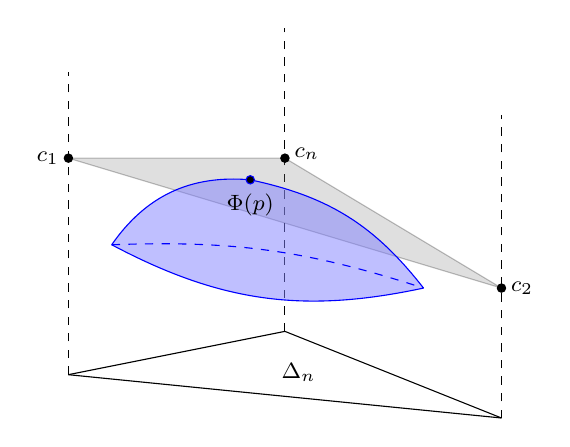
\begin{tikzpicture}[scale = 0.55]
%draw simplex
\draw (0, 0) to (5, 1);
\draw (5, 1) to (10, -1);
\draw (10, -1) to (0, 0);

%draw vertical lines
\draw[dashed] (0, 0) to (0, 7);
\draw[dashed] (5, 1) to (5, 8);
\draw[dashed] (10, -1) to (10, 6);

%draw hyperplane
%\draw [draw=black, fill=gray, opacity=0.25] (0,2) -- (5,7) -- (10,3) -- cycle;
\draw [draw=black, fill=gray, opacity=0.25] (0,5) -- (5,5) -- (10,2) -- cycle;
%\draw [blue, thick] plot [smooth] coordinates {(1,3) (4.2, 4.5) (8, 2)};

%draw graph
\path[fill=blue!50,opacity=.5] (1, 3) to [bend left=30] (4.2, 4.5) to [bend left=20] (8.2, 2) to [bend left=20] (1, 3);
\draw[blue] (1, 3) to [bend left=30] (4.2, 4.5);
\draw[blue] (4.2, 4.5) to [bend left=20] (8.2, 2);
\draw[blue] (8.2, 2) to [bend left = 20] (1, 3);
\draw[blue, dashed] (1, 3) to [bend left=10] (8.2, 2);

\node[circle, draw = black, fill = black,  inner sep=0pt, minimum size=3pt] at (0, 5) {};
\node[circle, draw = black, fill = black,  inner sep=0pt, minimum size=3pt] at (10, 2) {};
\node[circle, draw = black, fill = black,  inner sep=0pt, minimum size=3pt] at (5, 5) {};
\node [black, left] at (0, 5) {{\footnotesize $c_1$}};
\node [black, right] at (10, 2) {{\footnotesize $c_2$}};
\node [black, right] at (5, 5.1) {{\footnotesize $c_n$}};
\node [black, right] at (4.7, 0.06) {{\footnotesize $\Delta_n$}};

\node[circle, draw=blue, fill = black, inner sep=0pt, minimum size=3pt, label = below: {\footnotesize $\Phi(p)$}] at (4.2, 4.5) {};
\end{tikzpicture}
\caption{Geometric interpretation of multiplicatively generated portfolio.} \label{fig:fgp1}
\end{figure}

The following is the main result about multiplicatively generated portfolios. As this result is fundamental let us give a complete proof which also motivates the definition of the $L$-divergence. We also note that this proof is more transparent than the original proof (see \cite[Theorem 3.1.5]{F02} which is formulated in continuous time).

\begin{theorem} [Multiplicative decomposition] \cite{F99, PW15} \label{thm:fernholz}
Let $\eta$ be the trading strategy generated multiplicatively by the exponentially concave function $\varphi$ as in Definition \ref{def:multiplicative.fgp}. Then the value process of $\eta$ satisfies the decomposition
\begin{equation} \label{eqn:multiplicative.decomp}
\log V_{\eta}(t) - \log V_{\eta}(0) = \varphi(\mu(t)) - \varphi(\mu(0)) + \sum_{s = 0}^{t - 1} {\bf D}^{(1)} \left[ \mu(s + 1) \mid \mu(s)\right],
\end{equation}
where ${\bf D}^{(1)}\left[ \cdot \mid \cdot\right]$ is the $L^{(1)}$-divergence of $\varphi$ defined by \eqref{eqn:L.divergence}.
\end{theorem}
\begin{proof}
Using the multiplicative representation \eqref{eqn:V.multiplicative}, we have
\[
\frac{V_{\eta}(s + 1)}{V_{\eta}(s)} = \sum_{i = 1}^n \boldsymbol{\pi}_i(\mu(s)) \frac{\mu_i(s + 1)}{\mu_i(s)}.
\]
From \eqref{eqn:multiplicative.map}, we have
\[
\frac{\boldsymbol{\pi}_i(\mu(s))}{\mu_i(s)} = 1 + D_{e_i - \mu(s)} \varphi(\mu(s)),
\]
so we get the useful identity
\begin{equation} \label{eqn:multiplicative.derivative.identity}
\begin{split}
\frac{V_{\eta}(s + 1)}{V_{\eta}(s)} &= 1 + \sum_{i = 1}^n \mu_i(s + 1) D_{e_i - \mu(s)} \varphi(\mu(s))\\
&= 1 + D_{\mu(s + 1) - \mu(s)} \varphi(\mu(s)) \\
 &= 1 + \nabla \varphi(\mu(s)) \cdot (\mu(s + 1) - \mu(s)).
\end{split}
\end{equation}
Here we think of the gradient $\nabla \varphi(\mu(s))$ as operating on tangent vectors of $\Delta_n$. Financially, \eqref{eqn:multiplicative.derivative.identity} says that the relative return $(V_{\eta}(s + 1) - V_{\eta}(s))/V_{\eta}(s)$ of the portfolio is nothing but the directional derivative of $\varphi$.

By the concavity of $\Phi = e^{\varphi}$, for any $p, q \in \Delta_n$ we have
\[
\Phi(p) + \nabla \Phi(p) \cdot (q - p) \geq \Phi(q).
\]
Rewriting the inequality in terms of $\varphi$ and taking logarithm on both sides, we have
\[
{\bf D}^{(1)}[q \mid p] = \log \left( 1 + \nabla \varphi(p) \cdot (q - p) \right) - \left( \varphi(q) - \varphi(p) \right) \geq 0.
\]

Taking logarithm on both sides of \eqref{eqn:multiplicative.derivative.identity} and rearranging, we get
\[
\log V_{\eta}(s + 1) - \log V_{\eta}(s) = \varphi(\mu(s + 1)) - \varphi(\mu(s)) + {\bf D}^{(1)}[ \mu(s + 1) | \mu(s)].
\]
Summing over time gives the decomposition \eqref{eqn:multiplicative.decomp}.
\end{proof}

From \eqref{eqn:multiplicative.decomp}, the performance of the portfolio relative to the market can be attributed to two quantities. The first is the change in the market diversity $\varphi(\mu)$. It depends only on the beginning location $\mu(0)$ and the current location $\mu(t)$ of the market. Note that a change in $\varphi(\mu(t))$ is only caused by the component of market movement along the direction of $\nabla \varphi(\mu(t))$ which is perpendicular to the level set of $\varphi$. In particular, displacement along the same level set is not visible in this first term. The second term in \eqref{eqn:multiplicative.decomp} measures the volatility of the market, as it travels from $\mu(0)$ to $\mu(t)$, by the sum of ${\bf D}^{(1)}\left[ \mu(s + 1) \mid \mu(s) \right]$ over time. Intuitively, the functionally generated trading strategy $\eta$ outperforms the market if and only if the volatility is greater than the change in market diversity. In SPT, this decomposition allows one to formulate conditions under which relative arbitrage (with respect to the market portfolio) exists. Here is the simplest version of this idea:

\begin{proposition} [Relative arbitrage] \label{prop:relative.arbitrage}
Fix a smooth, exponentially concave function $\varphi: \Delta_n \rightarrow \mathbb{R}$. Let $M > 0$ be a constant and let $T > 0$ be a finite time horizon.  We say that a market weight sequence $\{\mu(t)\}_{t = 0}^{\infty}$ satisfies property $\mathcal{P}$ if $\varphi(\mu(t)) - \varphi(\mu(0)) > -M$ for all $t$ and $\sum_{s =0}^{T - 1} {\bf D}^{(1)} [ \mu(s + 1) | \mu(s) ] > M$, where ${\bf D}^{(1)}$ is the $L^{(1)}$-divergence of $\varphi$.  Then there exists an all-long trading strategy $\eta$ such that $V_{\eta}(T)/V_{\eta}(0) > 1$ (i.e., the strategy outperforms the market over the horizon $[0, T]$) for all market weight sequences satisfying property $\mathcal{P}$.
\end{proposition}
\begin{proof}
Let $\eta$ be the trading strategy generated multiplicatively by $\varphi$. By Theorem \ref{thm:fernholz}, if the market weight sequence satisfies property $\mathcal{P}$, we have
\begin{equation*}
\begin{split}
\log V_{\eta}(T) - \log V_{\eta}(0) &= \varphi(\mu(t)) - \varphi(\mu(0)) + \sum_{s = 0}^{t - 1} {\bf D}^{(1)} \left[ \mu(s + 1) \mid \mu(s)\right] \\
  &> -M + M = 0.
\end{split}
\end{equation*}
\end{proof}

The proof of Proposition \ref{prop:relative.arbitrage} is almost trivial because we already have the concept of multiplicatively generated portfolio. Without knowing this construction, it is not immediate why a relative arbitrage exists and how it is constructed. The usefulness of this result comes from the following observations (see \cite{F02}). Consider the {\it capital distribution} of the market defined by the reversed order statistics of the components of $\mu(t)$:
\[
\mu_{(1)}(t) \geq \mu_{(2)}(t) \geq \cdots \geq \mu_{(n)}(t).
\]
\begin{figure}[t!]
\centering
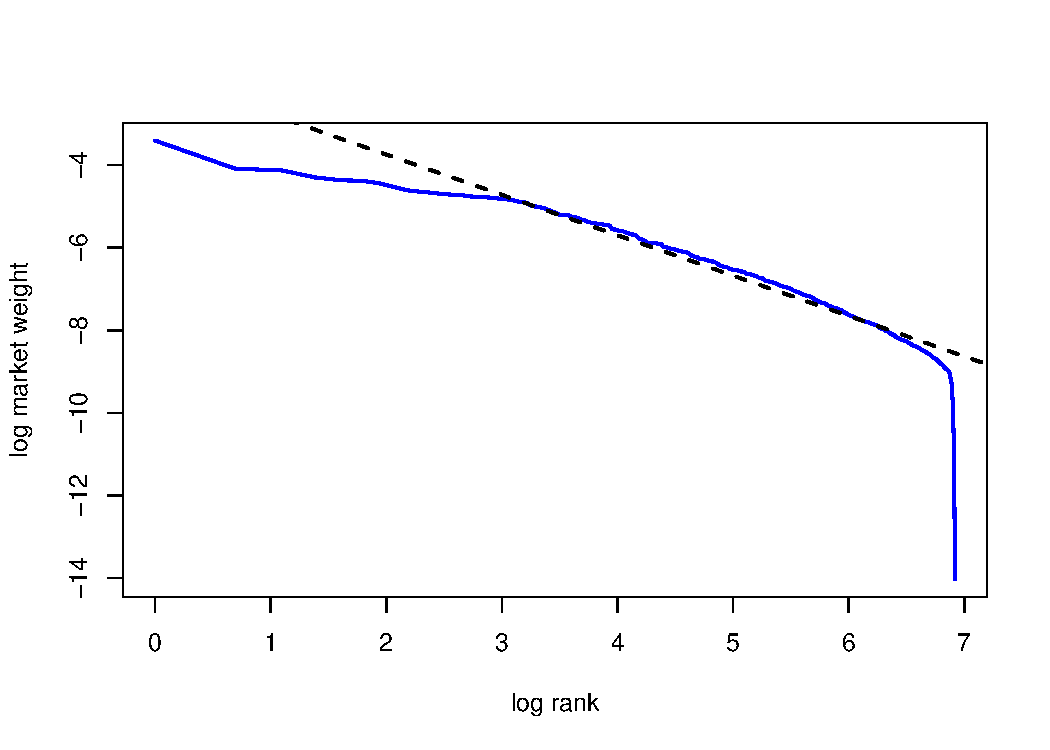
\includegraphics[scale=0.42]{capdist.pdf}
\caption{Capital distribution of the Russel 1000 Index in June 2015 (taken from \cite{P16}).} \label{fig:capdist}
\end{figure}
Empirically, it is found that if one plots $\log \mu_{(k)}(t)$ against $\log k$ (log of the rank), one gets an approximately linear curve (except the tail) which is relatively stable over time (see Figure \ref{fig:capdist}). This means that the capital distribution has an approximate Pareto distribution, and the market diversity $\varphi(\mu(t))$ is mean-reverting for $\varphi$ suitably chosen. On the other hand, for a typical $\varphi$ the market volatility $\sum_{s =0}^{T - 1} {\bf D} [ \mu(s + 1) | \mu(s) ]$ grows roughly linearly in time \cite{FK05}. Thus, it appears that the market satisfies the conditions of \eqref{prop:relative.arbitrage}.

The stability of the capital distribution has inspired many works on the construction and analysis of market models that exhibit such behaviors. Mathematically, these are systems of Brownian particles (representing the market capitalizations) where the drift and volatility coefficients depend on their relative rankings, and so they are called {\it rank-based models}. For more details we refer the reader to the papers \cite{BFK05, IPBKF11, P11, IPS13, FIK13, JR15, DT17} and their references.

Proposition \ref{prop:relative.arbitrage} only addresses long term relative arbitrages. In practice, {\it short term} relative arbitrages are much more relevant and interesting. Naturally their constructions require more work and conditions  (see  for example \cite{FKK05, BF08, FK:10, P16}). In particular, the paper \cite{FKR17} proves that market volatility alone does not imply the existence of short term relative arbitrage (this problem had been open in SPT for more than 10 years).

\subsection{Examples}
We give some examples of exponentially concave functions on $\Delta_n$, the portfolios they generate as well as the corresponding $L^{(1)}$-divergences.

\begin{example}[Constant-weighted portfolio]
Fix a probability vector $\pi \in \overline{\Delta}_n$ and consider the function 
\[
\varphi(p) = \sum_{j = 1}^n \pi_j \log p_j.
\]
It is exponentially concave since $\Phi = e^{\varphi} = \left(p_1\right)^{\pi_1} \cdots \left(p_n\right)^{\pi_n}$, the geometric mean with weights $\pi_1, \ldots, \pi_n$, is concave on $\Delta_n$. This function generates the constant-weighted portfolio $\boldsymbol{\pi}(p) \equiv \pi$, and the $L^{(1)}$-divergence is the excess growth rate ${\bf T}_{\pi}\left[q \mid p\right]$ given by \eqref{eqn:excess.growth}. We also observe that
\begin{equation*}
\begin{split}
\varphi(\mu(t)) - \varphi(\mu(0)) &= \sum_{j = 1}^n \pi_j \log \frac{\pi_j}{\mu_j(0)} - \sum_{j = 1}^n \pi_j \log \frac{\pi_j}{\mu_j(t)} \\
  &= H\left( \pi \mid \mu(0)\right) - H\left( \pi \mid \mu(t)\right)
\end{split}
\end{equation*}
is the negative of the change in the relative entropy $H\left( \pi \mid \cdot\right)$. In \cite{PW13}, we call the decomposition \eqref{eqn:multiplicative.decomp} for this portfolio the {\it energy-entropy decomposition}.
\end{example}

\begin{example}[Diversity-weighted portfolio] \label{eg:diversity}
For $\lambda \in (0, 1)$ fixed, let $\varphi$ be the function
\[
\varphi(p) = \frac{1}{\lambda} \log \sum_{j = 1}^n (p_j)^{\lambda},
\]
which is the logarithm of the function $\Phi$ given by \eqref{eqn:diversity}. Then $\varphi$ is exponentially concave and generates the {\it diversity-weighted portfolio} where
\begin{equation} \label{eqn:diversity.weighted.portfolio}
\boldsymbol{\pi}_i(p) = \frac{(p_i)^{\lambda}}{\sum_{j = 1}^n (p_j)^{\lambda}}, \quad i = 1, \ldots, n.
\end{equation}
Note that this portfolio interpolates between the equal-weighted portfolio $\boldsymbol{\pi}(p) \equiv \overline{e}$ (when $\lambda \downarrow 0$) and the market portfolio $\boldsymbol{\pi}(p) \equiv p$ (when $\lambda \uparrow 1$). See \cite{VK15} where the diversity-weighted portfolio is studied for negative values of $\lambda$. We remark that these cover, except for the log case, portfolios constructed using {\it Tukey's transformation ladder}; for more details see \cite{ETM17} where an extensive empirical study is given.


For $\lambda \in (0, 1)$ fixed, let $p^{(\lambda)} \in \Delta_n$ be given by $\boldsymbol{\pi}(p)$ as in \eqref{eqn:diversity.weighted.portfolio}. In information geometry, $p^{(\lambda)}$ is called the $\lambda$-{\it escort distribution} corresponding to the distribution $p$ (see \cite[Section 4.3]{A16}). Using this terminology we may interpret the portfolio in terms of the R\'{e}nyi entropy and divergence.

\begin{proposition}
Let $0 < \lambda < 1$. For $p \in \Delta_n$, we have
\[
\varphi(p) = \frac{1}{\lambda} \log \left( \sum_{j = 1}^n (p_j)^{\lambda} \right) = (\alpha - 1) \mathbf{H}_{\alpha} (p^{(\lambda)}),
\]
where $\alpha := \frac{1}{\lambda} \in (1, \infty)$, $p^{(\lambda)}$ is the $\lambda$-escort distribution corresponding to $p$, and 
\[
\mathbf{H}_{\alpha}(r) := \frac{1}{1 - \alpha} \log \left( \sum_{j = 1}^n (r_j)^{\alpha}\right)
\]
is the R\'{e}nyi entropy of order $\alpha$.

Moreover, the $L^{(1)}$-divergence of $\varphi$ is given by
\begin{equation}
{\bf D}^{(1)}[q \mid p] = (\alpha - 1) {\bf D}_{\alpha} ( q^{(\lambda)} || p^{(\lambda)} ),
\end{equation}
where $\mathbf{D}_{\alpha}( \cdot || \cdot)$ is the R\'{e}nyi divergence of order $\alpha$ defined by
\begin{equation}
\mathbf{D}_{\alpha}(p || q) := \frac{1}{\alpha - 1} \log \left( \sum_{j = 1}^n (p_j)^{\alpha} (q_j)^{1 - \alpha}\right).
\end{equation}
\end{proposition}
\begin{proof}
This is a direct computation and we only give the proof of the first statement. Using the fact that $p = \left(p^{(\lambda)}\right)^{(1/\lambda)}$, we have
\begin{equation*}
\begin{split}
\frac{1}{\lambda} \log \left( \sum_{i = 1}^n p_j^{\lambda}\right) &= \frac{1}{\lambda} \log \left( \sum_{i = 1}^n   \left(\frac{\left( p_i^{(\lambda)} \right)^{1/\lambda} }{ \sum_{j = 1}^n \left( p_j^{(\lambda)} \right)^{1/\lambda}}\right)^{\lambda}\right) \\
  &= - \log \left( \sum_{j = 1}^n \left( p_j^{(\lambda)} \right)^{\frac{1}{\lambda}} \right) \\
  &= (\alpha - 1) \frac{1}{1 - \alpha} \log \left( \sum_{j = 1}^n \left( p_j^{(\lambda)} \right)^{\alpha} \right),
\end{split}
\end{equation*}
which is $\alpha - 1$ times the R\'{e}nyi entropy.
\end{proof}



\begin{corollary}  \label{cor:diversity.weighted}
Let $\lambda \in (0, 1)$ and $\alpha := \frac{1}{\lambda} \in (1, \infty)$. The relative value of the diversity-weighted portfolio with parameter $\lambda$ satisfies
\begin{equation*}
\begin{split}
& \log {V_{\eta}(t)}{V_{\eta}(0)}\\
&= (\alpha - 1) \left[ \mathbf{H}_{\alpha} \left( \mu^{(\lambda)}(t) \right) - \mathbf{H}_{\alpha} \left( \mu^{(\lambda)}(0) \right) + \sum_{s = 0}^{t - 1} \mathbf{D}_{\alpha} \left(\mu^{(\lambda)}(t + 1) \middle|\middle| \mu^{(\lambda)}(t)\right)\right].
\end{split}
\end{equation*}
\end{corollary}
\end{example}

Consider a portfolio manager who tries to optimize over the parameter $\lambda$ of a diversity-weighted portfolio. By Corollary \ref{cor:diversity.weighted}, this means comparing the dynamics of the market weight $\mu(t)$ using different $\lambda$-escort geometries of the simplex. In particular, it is well-known that the R\'{e}nyi divergence satisfies
\begin{equation} \label{eqn:Renyi.Taylor}
{\bf D}_{\alpha} \left(r + tv || r\right) = \frac{\alpha}{2} t^2 \|v\|_r^2 + O(|t|^3), \quad t \rightarrow 0,
\end{equation}
where $\| v\|_r^2 := \sum_{i = 1}^n v_i^2 / r_i$ is the Fisher information metric at the point $r$. This geometric viewpoint may lead to new statistical methods and algorithms. In this regard, let us mention the recent work \cite{MSZ18} which studies the dynamics of market diversity in the context of large rank-based models, as well as the paper \cite{AFF07} which proposes a model for predicting change in market diversity. More generally, optimization of functionally generated portfolio amounts to finding the geometry in which $\mu(t)$ has the least change in diversity and has the greatest cumulated volatility.


\subsection{Multiplicative cyclical monotonicity}
In this subsection we provide a financial argument, given in \cite{PW15}, that motivates the definition of multiplicatively generated portfolio. 

Let us restrict to all-long trading strategies defined by portfolio maps, i.e., the portfolio weights satisfies $\pi(t) = \boldsymbol{\pi}(\mu(t))$ where $\boldsymbol{\pi}: \Delta_n \rightarrow \overline{\Delta}_n$ is a fixed deterministic function. When is $\boldsymbol{\pi}$ able to profit from market volatility? Intuitively it should satisfy the following property. Let $O$ be a (small) neighborhood in the simplex $\Delta_n$, and suppose $\mu(t) \in O$ for all $t$. From the discussion in Section \ref{sec:main.idea} market diversity is stable. Then, we expect that the portfolio will outperform the market asymptotically as long as there is enough volatility. Specifically, it should outperform the market whenever it is periodic. This idea leads to the following definition.

\begin{definition}[multiplicative cyclical monotonicity (MCM)]
A portfolio map $\boldsymbol{\pi}: \Delta_n \rightarrow \overline{\Delta}_n$ is multiplicatively cyclical monotone if for any integer $m \geq 0$ and any cycle $\{\mu(t)\}_{t = 0}^m$ with $\mu(0) = \mu(m)$ we have $V_{\eta}(m) \geq 1$, i.e.,
\begin{equation} \label{eqn:mcm}
\prod_{t = 0}^{m - 1} \left( \boldsymbol{\pi}(\mu(t)) \cdot \frac{\mu(t + 1)}{\mu(t)}\right) \geq 1.
\end{equation}
\end{definition}

In \cite{PW15} we observed that this property characterizes the multiplicatively generated portfolio. The following result is the multiplicative analogue of Rockafellar's theorem which characterizes the subdifferentials of convex functions in terms of cyclical monotonicity \cite[Section 24]{R70}.

\begin{theorem}
Suppose the portfolio map $\boldsymbol{\pi}: \Delta_n \rightarrow \overline{\Delta}_n$ is continuous. Then it is multiplicatively cyclical monotone if and only if there exists a differentiable, exponentially concave function $\varphi: \Delta_n \rightarrow \mathbb{R}$ which generates $\boldsymbol{\pi}$ in the sense of \eqref{eqn:multiplicative.map}.
\end{theorem}
\begin{proof}
Let us provide a sketch of proof to illustrate the main idea. Continuity of $\boldsymbol{\pi}$ is included here only to simplify the statement (in the general case $\varphi$ is not necessarily differentiable and we need to use supergradients). Suppose $\boldsymbol{\pi}$ is generated by $\varphi$. Consider a market weight sequence with $\mu(m) = \mu(0)$. By the decomposition \eqref{eqn:multiplicative.decomp}, we have
\[
\log V_{\eta}(m) - \log V_{\eta}(0) = \sum_{t = 0}^{m - 1} {\bf D}^{(1)} \left[ \mu(t + 1) \mid \mu(t)\right] \geq 0.
\]
Thus $V_{\eta}(m) \geq 1$ and $\boldsymbol{\pi}$ is MCM.

Conversely, suppose that $\boldsymbol{\pi}$ is MCM. Consider the function $\varphi$ defined by
\begin{equation*}
\begin{split}
\varphi(p) &= \varphi(p_0) + \inf\left\{ \log V_{\eta}(t) - \log V_{\eta}(0)\right\} \\
  &= \varphi(p_0) + \inf \left\{ \sum_{s = 0}^{t-1} \log \left( \sum_{i = 1}^n \boldsymbol{\pi}_i(\mu(s))  \frac{\mu_i(s + 1)}{\mu_i(s)}\right) \right\},
\end{split}
\end{equation*}
where $p_0 \in \Delta_n$ is fixed, $\varphi(p_0) \in \mathbb{R}$ is arbitrary, and the infimum is taken over $t \geq 0$ and all market weight sequences $\{\mu(s)\}_{s = 0}^t$ for which $\mu(0) = p_0$ and $\mu(t) = p$. Then it can be shown that $\varphi$ is differentiable, exponentially concave, and generates the given portfolio map $\boldsymbol{\pi}$. It can be shown that the function $\varphi$ is unique up to an additive constant.
\end{proof}

Using this characterization, in \cite{PW15} we introduced a Monge-Kantorovich optimal transport problem and showed that the optimal coupling can be represented using exponentially concave functions and the portfolios they generate.

\section{Generalized functional portfolio generation} \label{sec:general.portfolio}
\subsection{Motivations}
As it turns out, Theorem \ref{thm:fernholz} is not the only way to generate a portfolio such that a pathwise decomposition holds. In \cite{KR17} Karatzas and Ruf introduced a novel {\it additive} generation and used it to construct relative arbitrages (see \cite{RX18} for another extension involving an additional finite variation process). The following result uses the terminology of \cite[Section 3.3]{V16} and adapts the construction to our discrete time setting. We omit the proof as it is contained (in the limit) in Theorem \ref{thm:general.decomp} below.

\begin{theorem} [Additively generated portfolio \cite{KR17}] \label{thm:additive.portfolio}
Let $\varphi: \Delta_n \rightarrow (0, \infty)$ be a smooth concave function and let $v_0 \in \mathbb{R}$ be an initial portfolio value. Then there is a self-financing trading strategy $\eta$ satisfying $V_{\eta}(0) = v_0$ and
\begin{equation} \label{eqn:additive.portfolio}
\eta_i (t) = D_{e_i - \mu(t)} \varphi(\mu(t)) + V_{\eta}(t), \quad i = 1, \ldots, n.
\end{equation}
Its relative value satisfies the decomposition
\begin{equation} \label{eqn:additive.decomp}
V_{\eta}(t) - V_{\eta}(0) = \varphi(\mu(t)) - \varphi(\mu(0)) + \sum_{s = 0}^{t - 1} {\bf D}^{(0)}  \left[\mu(t + 1) \mid \mu(t) \right],
\end{equation}
where ${\bf D}^{(0)}[ \cdot | \cdot]$ is the Bregman (or $L^{(0)}$) divergence of $\varphi$ as in \eqref{eqn:Bregman.divergence}. We call $\eta$ the strategy generated additively by $\varphi$.
\end{theorem}

Note that the additively generated portfolio involves a concave rather than exponentially concave function.

\begin{example} \label{eg:quadratic}
Consider the function
\[
\varphi(p) = \frac{-1}{2} |p|^2 = \frac{-1}{2} \left(p_1^2 + \cdots + p_n^2\right).
\]
It generates the trading strategy $\eta(t)$ given by $
\eta_i(t) = |p|^2 - p_i + V_{\eta}(t)$. It is interesting to note that the Bregman divergence of $\varphi$ is half of the squared Euclidean distance:
\[
{\bf D}^{(0)}\left[q \mid p\right] = \frac{1}{2} |p - q|^2.
\]
Thus the squared Euclidean distance indeed has a financial meaning for this specific trading strategy.
\end{example}

Observe that both the multiplicative and additive decompositions \eqref{eqn:multiplicative.decomp} and \eqref{eqn:additive.decomp} can be written in the form
\begin{equation} \label{eqn:general.decomp}
g(V_{\eta}(t)) - g(V_{\eta}(0)) = \varphi(\mu(t)) - \varphi(\mu(0)) + {\bf D}\left[\mu(t + 1) \mid \mu(t) \right],
\end{equation}
where $g$, $\varphi$ and ${\bf D}\left[ \cdot \mid \cdot\right]$ are suitable functions:
\begin{itemize}
\item (Multiplicative generation) $g(x) = \log x$ and ${\bf D}\left[ \cdot \mid \cdot\right]$ is the $L^{(1)}$-divergence of the exponentially concave function $\varphi$.
\item (Additive generation) $g(x) = x$ and ${\bf D}\left[ \cdot \mid \cdot\right]$ is the $L^{(0)}$-divergence of the concave function $\varphi$.
\end{itemize}


It is natural to ask if there exist other portfolio constructions that admit pathwise decompositions of the form \eqref{eqn:general.decomp}. To formulate this question rigorously we introduce the general concept of divergence.


\begin{definition}[Divergence on $\Delta_n$] \label{def:divergence}
A divergence on $\Delta_n$ is a non-negative functional ${\bf D}\left[ \cdot \mid \cdot \right] : \Delta_n \times \Delta_n \rightarrow [0, \infty)$ satisfying the following conditions:
\begin{itemize}
\item[(i)] \ ${\bf D}\left[ q \mid p\right] = 0$ if and only if $p = q$.
\item[(ii)] \  It admits a quadratic approximation of the form
\begin{equation} \label{eqn:Riemannian}
{\bf D}\left[p + \Delta p \mid p\right] = \frac{1}{2} \sum_{i, j = 1}^n g_{ij}(p) \Delta p_i \Delta p_j + O(| \Delta p |^3)
\end{equation}
as $|\Delta p| \rightarrow 0$, and the matrix $G(p) = \left( g_{ij}(p) \right)$ varies smoothly in $p$ and is strictly positive definite in the sense that
\begin{equation} \label{eqn:positive.definite}
\sum_{i, j = 1}^n g_{ij}(p) v_i v_j > 0
\end{equation}
for all vectors $v \in \mathbb{R}^n$ that are tangent to $\Delta_n$, i.e., $v_1 + \cdots + v_n = 0$.
\end{itemize}
If condition (i) is dropped and in \eqref{eqn:positive.definite} we do not strict inequality, we call ${\bf D}\left[ \cdot \mid \cdot \right]$ a pseudo-divergence.
\end{definition}

\begin{example}
Let $\Hess \varphi$ denote the Euclidean Hessian of $\varphi$. If $\alpha > 0$ and $\varphi$ is $\alpha$-exponentially concave, then its $L^{(\alpha)}$-divergence satisfies
\begin{equation} \label{eqn:L.alpha.approximation}
\begin{split}
& {\bf D}^{(\alpha)}\left[p + \Delta p \mid p \right] \\
&= \frac{-1}{2} (\Delta p)^{\top} \left( \Hess \varphi(p) + \alpha (\nabla \varphi(p))(\nabla \varphi(p) )^{\top}\right) (\Delta p) + O(|\Delta p|^3).
\end{split}
\end{equation}
If $\varphi$ is concave, then its $L^{(0)}$-divergence satisfies
\[
{\bf D}^{(0)}\left[p + \Delta p \mid p \right] = \frac{-1}{2} (\Delta p)^{\top} \Hess \varphi(p) (\Delta p) + O(|\Delta p|^3).
\]
It is easy to verify that the corresponding matrix $G(p)$ is semi-positive definite. They become true divergences if $\Hess e^{\alpha \varphi}$ and $\Hess \varphi$ respectively are strictly positive definite.
\end{example}

\begin{definition} [General functional portfolio construction] \label{def:generation}
Let $\eta = \{\eta(t)\}_{t = 0}^{\infty}$ be a self-financing trading strategy whose relative value process is $\{V_{\eta}(t)\}$, and let $\varphi, g: \Delta_n \rightarrow \mathbb{R}$ be functions on $\Delta_n$ where $g$ is strictly increasing. We say that  $\eta$ is generated by $\varphi$ with scale function $g$ if there exists a pseudo-divergence ${\bf D}[\cdot  : \cdot ]$ on $\Delta_n$ such that \eqref{eqn:general.decomp} holds for all market sequences $\{\mu(t)\}_{t = 0}^{\infty}$.
\end{definition}

In this section we will introduce a new $(\alpha, C)$-generation, and, after giving an empirical example, show that it characterizes all functional portfolio generation in the sense of Definition \ref{def:generation}. For expositional convenience we always assume that the generating function is smooth. Extension of this construction to continuous time is left for future research.

\subsection{A new functional portfolio generation}

\begin{theorem} [$(\alpha, C)$-generation] \label{thm:genera.generation}
Let $\alpha > 0$ and $C \geq 0$ be fixed parameters, and let $\varphi: \Delta_n \rightarrow \mathbb{R}$ be smooth and $\alpha$-exponentially concave. Then, for any given initial value $v_0 \in \mathbb{R}$, there exists a unique self-financing trading strategy $\eta(t)$ such that $V_{\eta}(0) = v_0$ and
\begin{equation} \label{eqn:general.generation}
\eta_i(t) = \alpha (C + V_{\eta}(t)) D_{e_i - \mu(t)} \varphi(\mu(t)) + V_{\eta}(t), \quad i = 1, \ldots, n,
\end{equation}
for all $t$. We call $\eta$ the strategy which is $(\alpha, C)$-generated by $\varphi$.
\end{theorem}
\begin{proof}
We will prove by induction on $T \geq 0$ that the statement holds on the time interval $[0, T]$. Consider $T = 0$. Let $V_{\eta}(0) = v_0$. If we define
\[
\eta_i(0) = \alpha (C + v_0) D_{e_i - \mu(0)} \varphi(\mu(t)) +  v_0,
\]
then, since $\sum_{i = 1}^n \mu_i (e_i - \mu) = 0$, we have
\[
\eta(0) \cdot \mu(0) = \alpha (C + v_0) \sum_{i = 1}^n \mu_i(0) D_{e_i - \mu(0)} \varphi(\mu(t)) +  \sum_{i = 1}^n \mu_i(0) v_0 = v_0.
\]
Thus there is a unique strategy $\eta$ which satisfies \eqref{eqn:general.generation} at time $0$.

Suppose by the induction hypothesis that the statement holds up to time $T$. Then $\eta(T)$ and $V_{\eta}(T)$ are uniquely defined, and the portfolio value at time $T + 1$ is given uniquely by
\begin{equation} \label{eqn:value.Tp1}
V_{\eta}(T + 1) := V_{\eta}(T) + \eta(T) \cdot (\mu(T + 1) - \mu(T)).
\end{equation}
Thus there is a unique vector $\eta(T + 1)$ satisfying \eqref{eqn:general.generation}. 

It remains to show that the strategy is self-financing at time $T + 1$, i.e., $\eta(T) \cdot \mu(T + 1) = \eta(T + 1) \cdot \mu(T + 1)$ (see \eqref{eqn:self.financed}). Using \eqref{eqn:general.generation}, we have
\begin{equation*}
\begin{split}
\eta(T + 1) \cdot \mu(T + 1) &= \sum_{i = 1}^n \mu_i(T + 1) \alpha (C + V_{\eta}(T + 1)) D_{e_i - \mu(T + 1)} \varphi(\mu(T + 1)) \\
&\quad + \sum_{i = 1}^n \mu_i(T + 1) V_{\eta}(T + 1) \\
&= V_{\eta}(T + 1) \quad \text{(since $\sum_{i = 1}^n \mu_i(T + 1) D_{e_i - \mu(T + 1)} = 0$)} \\
&= V_{\eta}(T) + \eta(T) \cdot (\mu(T + 1) - \mu(T)) \quad \text{(by \eqref{eqn:value.Tp1})} \\
&= \eta(T) \cdot \mu(T) + \eta(T) \cdot (\mu(T + 1) - \mu(T)) \\
&= \eta(T) \cdot \mu(T + 1).
\end{split}
\end{equation*}
In the second last equality we used the self-financing property up to time $T$. This proves that the strategy is uniquely defined at all times.
\end{proof}


In Theorem \ref{thm:general.decomp} we show that this trading strategy corresponds to the scale function given by\begin{equation} \label{eqn:general.scale.function}
g(x) = \frac{1}{\alpha} \log (C + x).
\end{equation}
Moreover, in Section \ref{sec:characterize} we show that up to an additive constant this function (together with $g(x) = x$) is the most general scale function. Comparing \eqref{eqn:general.generation} with \eqref{eqn:multiplicative.map} and \eqref{eqn:additive.portfolio}, we see that multiplicative generation corresponds to the case $C = 0$ and $\alpha = 1$, and additive generation corresponds to the limit when $\alpha = \frac{1}{C} \rightarrow 0$. 

The trading strategy $\eta$ given by \eqref{eqn:general.generation} can be interpreted as follows. 

\begin{lemma} [Portfolio weight of $\eta$]
Let $\pi^{(\alpha)}$ be the portfolio process generated multiplicatively by the $1$-exponentially concave function $\alpha \varphi$. If $V_{\eta}(t) > 0$, the portfolio weight vector $\pi(t)$ of the $(\alpha, C)$-generated trading strategy $\eta$ is given by
\begin{equation} \label{eqn:eta.weight}
\pi(t) = \left( \frac{\eta_1(t) \mu_1(t)}{V_{\eta}(t)}, \ldots, \frac{\eta_n(t) \mu_n(t)}{V_{\eta}(t)}\right) = \frac{C + V_{\eta}(t)}{V_{\eta}(t)} \pi^{(\alpha)}(t) - \frac{C}{V_{\eta}(t)} \mu(t).
\end{equation}
In particular, $\eta(t)$ longs the multiplicatively generated portfolio $\pi^{(\alpha)}$ and shorts the market portfolio with weights depending on $V_{\eta}(t)$ and $C$.
\end{lemma}
\begin{proof}
Direct computation using \eqref{eqn:general.generation}.
\end{proof}

By increasing $C$, we may construct portfolios that are more aggressive than the multiplicatively generated portfolio. Note that we keep the parameter $\alpha$ so that we can generate different portfolios with the same generating function $\varphi$ (as long as $e^{\alpha \varphi}$ is concave).

Next we show that the new portfolio generation admits a pathwise decomposition for the portfolio value.

\begin{theorem}[Pathwise decomposition] \label{thm:general.decomp}
Consider an $(\alpha, C$)-generated trading strategy $\eta$ as in Theorem \ref{thm:genera.generation}. If $V_{\eta}(\cdot) > -C$, then the value process satisfies the pathwise decomposition
\begin{equation} \label{eqn:new.decomp}
\frac{1}{\alpha} \log \frac{C + V_{\eta}(t)}{C + V_{\eta}(0)} = \varphi(\mu(t)) - \varphi(\mu(0)) + \sum_{s = 0}^{t - 1} {\bf D}^{(\alpha)}  \left[ \mu(s + 1) \mid \mu(s) \right],
\end{equation}
where ${\bf D}^{(\alpha)}$ is the $L^{(\alpha)}$-divergence of $\varphi$.
\end{theorem}
\begin{proof}
The proof is similar to that of Theorem \ref{thm:fernholz}. By \eqref{eqn:general.generation}, for each time $t$ we have
\begin{equation} \label{eqn:general.decomp.proof}
\begin{split}
& \frac{1}{\alpha} \log (C + V_{\eta}(t + 1)) - \frac{1}{\alpha} \log (C + V_{\eta}(t))\\
 &= \frac{1}{\alpha} \log \frac{C + V_{\eta}(t) + \alpha (C + V_{\eta}(t)) \nabla \varphi(\mu(t)) \cdot (\mu(t + 1) - \mu(t))}{C + V_{\eta}(t)} \\
 &= \frac{1}{\alpha} \log \left(1 + \alpha \nabla \varphi(\mu(t)) \cdot (\mu(t + 1) - \mu(t))\right) \\
 &= \varphi(\mu(t + 1)) - \varphi(\mu(t)) + {\bf D}^{(\alpha)} \left[\mu(t + 1) \mid \mu(t)\right].
\end{split}
\end{equation}
This yields the desired decomposition. The condition $V_{\eta}(\cdot) > -C$ is imposed so that the logarithms make sense.
\end{proof}

\subsection{An empirical example}

Consider a smooth and exponentially concave function $\varphi$. It is $\alpha$-exponentially concave for all $0 < \alpha \leq 1$ and is concave (which corresponds to the case $\alpha \downarrow 0$). Thus both the additive and multiplicatively generated portfolios are well-defined. Unfortunately, while the $L^{(\alpha)}$-divergence is a natural interpolation,  there does not seem to be a canonical choice for the constant $C$ that connects the two basic cases.

 In this example we consider instead the parameterized family $\{ \eta^{(\alpha)} \}_{0 \leq \alpha \leq 1}$ where $\eta^{(\alpha)}$ is the trading strategy $(\alpha, \frac{1}{\alpha})$-generated by $\varphi$ (so when $\alpha = 0$ it is the additively generated portfolio), and compare their empirical performance. We set $V_{\eta^{(\alpha)}}(0) = 1$ for all $\alpha$.  Note that $\eta^{(1)}$ is not the multiplicatively generated portfolio as it also shorts the market portfolio.

Consider as in Figure \ref{fig:simplex} the (beginning) monthly stock prices of the US companies Ford, Walmart and IBM from January 1990 ($t = 0$) to  September 2017 ($t = 332$). We normalize the prices so that at $t = 0$ the market weight is at the barycenter $\left(\frac{1}{3}, \frac{1}{3}, \frac{1}{3}\right)$. The path of the market weight $\mu(t)$ in the simplex $\Delta_3$ is plotted in Figure \ref{fig:simplex} (right).

\begin{figure}[t!]
\centering
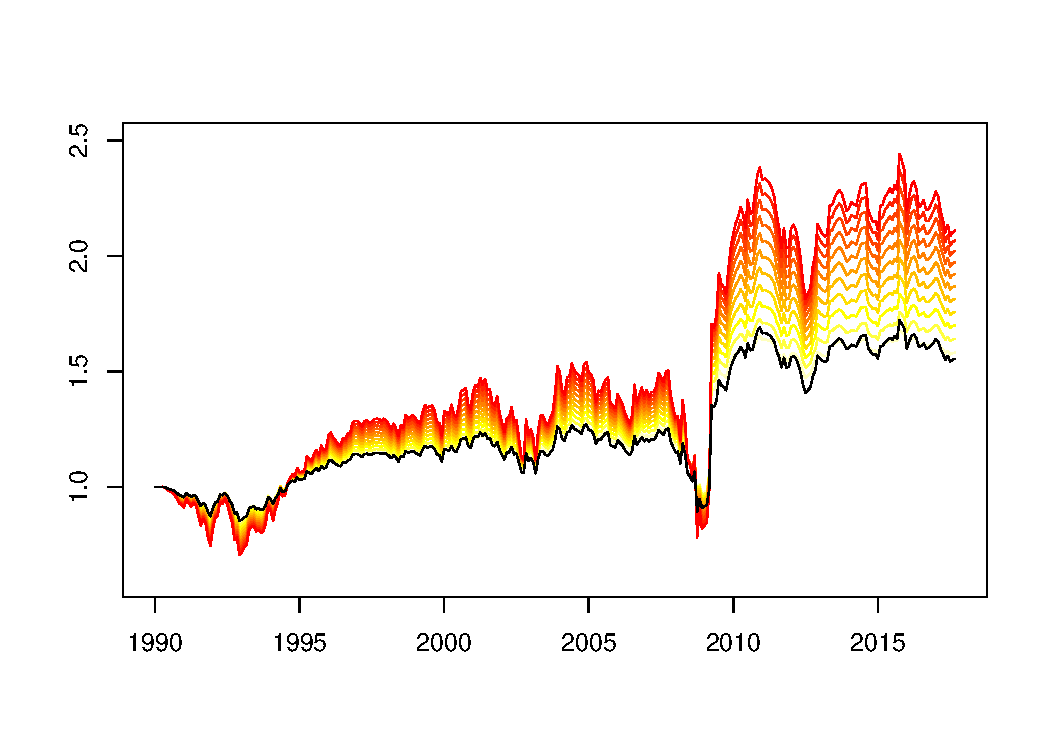
\includegraphics[scale=0.5]{simulation.pdf}
\caption{Time series of the relative portfolio value $V_{\eta^{(\alpha)}}(t)$, from $\alpha = 0$ (yellow) to $\alpha = 1$ (red). The value of the equal-weighted portfolio is shown in black.}
\label{fig:output}
\end{figure}

We consider the $1$-exponentially concave function
\begin{equation}
\varphi(p) = \sum_{i = 1}^3 \frac{1}{3} \log p_i
\end{equation}
which generates multiplicatively the equal-weighted portfolio $\boldsymbol{\pi}(p) \equiv \overline{e} = \left(\frac{1}{3}, \frac{1}{3}, \frac{1}{3}\right)$. By \eqref{eqn:general.generation}, for each $\alpha \in [0, 1]$ the trading strategy is given by
\[
\eta^{(\alpha)}_i(t) = \left(1 + \alpha V_{\eta}(t)\right) \left(\frac{1}{3 \mu_i(t)} - 1\right) + V_{\eta}(t).
\]
In terms of portfolio weights, we have
\[
\pi^{(\alpha)}(t) = \frac{1 + \alpha V_{\eta}(t)}{V_{\eta}(t)} \overline{e} - \frac{1 + \alpha V_{\eta}(t) - V_{\eta}(t)}{V_{\eta}(t)} \mu(t).
\]
Thus the portfolio longs more and more the equal-weighted portfolio as $\alpha$ increases. The corresponding $L^{(\alpha)}$-divergence is given by
\[
{\bf D}^{(\alpha)}\left[q \mid p\right] = \frac{1}{\alpha} \log \left(1 + \alpha \sum_{i = 1}^n \frac{1}{n p_i} (q_i - p_i)\right) - \sum_{i = 1}^n \frac{1}{n} \log \frac{q_i}{p_i}.
\]

The relative values of the simulated portfolios are plotted in Figure \ref{fig:output}. At the end of the period the portfolio value is increasing in $\alpha$, and the additive portfolio ($\alpha = 0$) has the smallest value. It is interesting to note that the reverse is true at the beginning. Note that the values fluctuate widely in the period 2008--2009 corresponding to the financial crisis. For comparison, we also simulate the multiplicatively generated equal-weighted portfolio (i.e., $(\alpha, C) = (1, 0)$) and plot the result in  Figure \ref{fig:output}. Surprisingly the additive and multiplicative portfolios have similar behaviors here. In this period, shorting the market by using a positive value for $C$ gives significant advantage over both the additive and multiplicative portfolios. Dynamic optimization over our extended functionally generated portfolios is an interesting problem.


\subsection{Characterizing functional portfolio generation} \label{sec:characterize}
Now we show that our $(\alpha, C)$-generation is the most general one. Throughout this subsection we let $\eta$ be a functionally generated trading strategy as in Definition \ref{def:generation}. We assume that the scale function $g$ is smooth and $g'(x) > 0$ for all $x$. We also require that the domain of $g$ contains the positive real line $(0, \infty)$. Furthermore, we assume that $\varphi$ is smooth, and $\eta$ is non-trivial in the sense that for all $t \geq 0$ and all market weight paths $\{\mu(s)\}_{s = 0}^t$ up to time $t$, the profit-or-loss
\[
V_{\eta}(t + 1) - V_{\eta}(t) = \eta(t) \cdot (\mu(t + 1) - \mu(t))
\]
is not identically zero as a function of $\mu(t + 1) \in \Delta_n$. For technical reasons we also assume that for any $x > 0$, there exists $t \geq 0$ and a sequence $\{\mu(s)\}_{s = 0}^t$ such that $V_{\eta}(t) = x$.

\begin{theorem} \label{thm:scale.function}
Under the above conditions, the scale function has one of the following forms.  Either
\begin{equation} \label{eqn:shape1}
g(x) = c_1 x + c_2
\end{equation}
where $c_1 > 0$ and $c_2 \in \mathbb{R}$, or
\begin{equation} \label{eqn:shape2}
g(x) = c_2 \log(c_1 + x) + c_3
\end{equation}
where $c_1 \geq 0$, $c_2 > 0$ and $c_3 \in \mathbb{R}$. In the first case $\varphi$ is concave and $\eta$ is additively generated by $\varphi$, whereas in the second case $\varphi$ is $\alpha$-exponentially concave with $c_2 = \frac{1}{\alpha}$ and $\eta$ is $(\alpha, c_1)$-generated by $\varphi$. The corresponding pseudo-divergence is the $L^{(\alpha)}$-divergence of $\varphi$.
\end{theorem}

Note that in \eqref{eqn:shape1} and \eqref{eqn:shape2} the additive constants are irrelevant and may be discarded. We will prove Theorem \ref{thm:scale.function} with several lemmas. First we observe that the decomposition \eqref{eqn:general.decomp} already implies a formula of the trading strategy.

\begin{lemma}
For any $t$ and any tangent vector $v$ of $\Delta_n$ (i.e., $v_1 + \cdots + v_n = 0$) we have
\begin{equation} \label{eqn:eta.as.gradient}
\eta(t) \cdot v  =  \frac{1}{g'(V_{\eta}(t))} \nabla \varphi(\mu(t)) \cdot  v.
\end{equation}
In particular, for each $i = 1, \ldots, n$ we have
\begin{equation} \label{eqn:eta.formula}
\eta_i(t) = \frac{1}{g'(V_{\eta}(t))} D_{e_i - \mu(t)} \varphi(\mu(t)) + V_{\eta}(t).
\end{equation}
\end{lemma}
\begin{proof}
From \eqref{eqn:general.decomp} we have the identity
\begin{equation} \label{eqn:1step.decomp}
g(V_{\eta}(t + 1)) - g(V_{\eta}(t)) = \varphi(\mu(t + 1)) - \varphi(\mu(t)) + {\bf D}\left[ \mu(t + 1) \mid \mu(t) \right]
\end{equation}
which holds for all values of $\mu(t + 1)$. Write
\[
V_{\eta}(t + 1) = V_{\eta}(t) + \eta(t) \cdot (\mu(t + 1) - \mu(t))
\]
and let $\mu(t + 1) - \mu(t) = \delta v$, $\delta > 0$ sufficiently small, and compute the first order approximation of both sides of \eqref{eqn:1step.decomp}. Since ${\bf D}\left[ \cdot \mid \cdot \right]$ is a pseudo-divergence, by \eqref{eqn:Riemannian} its first order approximation vanishes. Evaluating the derivatives and dividing by $\delta > 0$, we obtain \eqref{eqn:eta.as.gradient}.

Letting $v = e_i - \mu(t)$ in \eqref{eqn:eta.formula} for $i = 1, \ldots, n$, we get the formula \eqref{eqn:eta.formula}.
\end{proof}

Observe that \eqref{eqn:eta.as.gradient} reduces to \eqref{eqn:additive.portfolio} when $g(x) = x$, and to \eqref{eqn:multiplicative.map} when $g(x) = \log x$. Also, we note that $\eta(t)$ depends only on $\mu(t)$ and the current portfolio value $V_{\eta}(t)$. Putting $v = \mu(t + 1) - \mu(t)$ in \eqref{eqn:eta.as.gradient}, we have
\begin{equation} \label{eqn:for.use}
V_{\eta}(t + 1) - V_{\eta}(t) = \frac{1}{g'(V_{\eta}(t))}\nabla \varphi(\mu(t)) \cdot (\mu(t + 1) - \mu(t)).
\end{equation}

Consider the expression
\begin{equation} \label{eqn:gV.expression}
\begin{split}
& g(V_{\eta}(t + 1)) - g(V_{\eta}(t))\\
&= g\left(V_{\eta}(t) + \left[V_{\eta}(t + 1) - V_{\eta}(t)\right]\right) - g(V_{\eta}(t)) \\
  &= g\left(V_{\eta}(t) + \frac{1}{g'(V_{\eta})}  \nabla \varphi(\mu(t)) \cdot ( \mu(t + 1) - \mu(t))\right) - g(V_{\eta}(t)).
\end{split}
\end{equation}
By \eqref{eqn:general.decomp}, this equals
\[
\varphi(\mu(t + 1)) - \varphi(\mu(t)) + {\bf D}[\mu(t + 1) | \mu(t)],
\]
which is a function of $\mu(t)$ and $\mu(t + 1)$ only. Thus, the expression in \eqref{eqn:gV.expression} does not depend on the current portfolio value $V_{\eta}(t)$. From this observation we will derive a differential equation satisfied by $g$.

\begin{lemma} 
The scale function $g$ satisfies the third order nonlinear ODE
\begin{equation} \label{eqn:ODE1}
g' g''' =2  (g'')^2
\end{equation}
on the positive real line $(0, \infty)$.
\end{lemma}
\begin{proof}
Given $x > 0$, write $x = V_{\eta}(t)$ for some $t \geq 0$ and market sequence $\{\mu(s)\}_{s = 0}^t$. Let $\delta =  \nabla \varphi(\mu(t)) \cdot ( \mu(t + 1) - \mu(t) )$. From \eqref{eqn:gV.expression}, for any $\delta$, the expression
\begin{equation} \label{eqn:invariance}
g(x + \frac{1}{g'(x)} \delta) - g(x)
\end{equation}
does not depend on $x$.

Differentiating \eqref{eqn:invariance} with respect to $x$, we have
\[
g'(x + \frac{1}{g'(x)}\delta) \left(1 - \delta \frac{g''(x)}{(g'(x))^2}\right) - g'(x) = 0.
\]
Next we differentiate with respect to $\delta$ (since $\eta$ is assumed to be non-trivial, this can be done by varying $\mu(t + 1)$):
\[
g''(x + \frac{1}{g'(x)} \delta) \frac{1}{g'(x)} \left(1 - \delta \frac{g''(x)}{(g'(x))^2}\right) + g'(x + \frac{1}{g'(x)} \delta) \frac{- g''(x)}{(g'(x))^2} = 0.
\]
Differentiating one more time with respect to $\delta$, we have
\begin{equation*}
\begin{split}
& g'''(x + \frac{1}{g'(x)}\delta) \frac{1}{(g'(x))^2} \left(1 - \delta \frac{g''(x)}{(g'(x))^2}\right)\\
&\quad + g''(x + \frac{1}{g'(x)} \delta) \frac{-g''(x)}{(g'(x))^3} - \frac{g''(x + \frac{1}{g'(x)} \delta) g''(x)}{(g'(x))^3} = 0.
\end{split}
\end{equation*}
Setting $\delta = 0$, we get $\frac{g'''(x)}{(g'(x))^2} - 2 \frac{(g''(x))^2}{(g'(x))^3} = 0$ which gives the ODE \eqref{eqn:ODE1}. (Note that we assumed that $g'(x) > 0$ for all $x$.)
\end{proof}

With the differential equation in hand, it is not difficult to find the general solutions. They can be verified using direct substitution and the local uniqueness of the autonomous equation.

\begin{lemma} \label{lem:ODE.solution}
All solutions to the ODE \eqref{eqn:ODE1} can be written in the form
\begin{equation} \label{eqn:g.equation}
g(x) = c_0 + c_1 x  \quad \text{or} \quad  g(x) = c_2 \log (c_1 + x) + c_3,
\end{equation}
where the $c_i$'s are real constants. The constraints on the constants stated in Theorem \ref{thm:scale.function} follow from our assumptions of $g$.
\end{lemma}

Now we are ready to complete the proof of Theorem \ref{thm:scale.function}. By Lemma \ref{lem:ODE.solution}, the scale function (up to an additive constant which is irrelevant) has the form \eqref{eqn:shape1} or \eqref{eqn:shape2}. Consider the second case (the first case is similar). Then by \eqref{eqn:for.use},  \eqref{eqn:gV.expression} and the third equality of \eqref{eqn:general.decomp.proof} (which does not depend on $\alpha$-exponential concavity of $\varphi$), for any $p = \mu(s)$ and $q = \mu(s + 1)$, we have
\[
{\bf D}\left[q \mid p\right] = \frac{1}{\alpha} \log \left( 1 + \alpha \nabla \varphi(p) \cdot (q - p)\right) - \left( \varphi(q) - \varphi(p)\right)
\]
which is exactly the expression of the $L^{(\alpha)}$-divergence. By assumption ${\bf D}\left[\cdot \mid \cdot\right]$ is a pseudo-divergence so it is non-negative for all $p$, $q$. It is easy to check that this implies that $\varphi$ is $\alpha$-exponentially concave, and so $\eta$ is the $(\alpha, c_1)$-generated trading strategy.



\section{Further properties of $L$-divergence} \label{sec:futher}
In this section we gather some further properties of $L$-divergence and describe some related problems. For simplicity we focus on the $L^{(1)}$-divergence, and refer the reader to \cite{W17b} for a systematic study of the $L^{(\alpha)}$-divergence. We always assume that the generating functions are smooth. It is clear that some of the problems make sense on domains other than the unit simplex.

\subsection{Interpolation and comparison}
If $\varphi^{(0)}$ and $\varphi^{(1)}$ are exponentially concave functions on $\Delta_n$, by the inequality of the arithmetic and geometric means, we have that
\[
\varphi^{(\lambda)} := (1 - \lambda) \varphi^{(0)} + \lambda \varphi^{(1)}
\]
is exponentially concave for any $0 < \lambda < 1$. If $\boldsymbol{\pi}^{(0)}$ and $\boldsymbol{\pi}^{(1)}$ are the portfolio maps generated multplicatively by $\varphi^{(0)}$ and $\varphi^{(1)}$ respectively, then $\varphi^{(\lambda)}$ generates the portfolio map
\[
\boldsymbol{\pi}^{(\lambda)}(\cdot) \equiv (1 - \lambda) \boldsymbol{\pi}^{(0)}(\cdot) + \lambda \boldsymbol{\pi}^{(1)}(\cdot),
\]
which is a constant-weighted portfolio of $\boldsymbol{\pi}^{(0)}$ and $\boldsymbol{\pi}^{(1)}$ \cite[Lemma 4.4]{W15}. Thus, the spaces of exponentially concave functions and MCM portfolio maps (see Definition \ref{def:multiplicative.fgp}) are convex. Moreover, the $L$-divergence ${\bf D}^{(1)}\left[ \cdot \mid \cdot\right]$ is concave in the function $\varphi$. In \cite{PW16}, this interpolation provides a new displacement interpolation for a logarithmic optimal transport problem.

Let ${\bf D}_{\varphi}$ and ${\bf D}_{\psi}$ be the $L$-divergences generated respectively by the exponentially concave functions $\varphi$ and $\psi$, we say that ${\bf D}_{\psi}$ {\it dominates} ${\bf D}_{\varphi}$ if 
\begin{equation} \label{eqn:domination}
{\bf D}^{(1)}_{\psi}\left[ q \mid p\right] \geq {\bf D}^{(1)}_{\varphi}\left[ q \mid p\right]
\end{equation}
for all $p, q \in \Delta_n$. Financially, this means that the portfolio generated by $\psi$ captures more volatility than the one generated by $\varphi$. An interesting problem is to find the maximal elements in this partial order, and the following result is obtained in \cite{W15} using the relative convexity lemma in \cite{CDO07}.

\begin{theorem} \label{thm:maximal}
Suppose $\varphi$ is symmetric, i.e., $\varphi(p_1, \ldots, p_n) = \varphi(p_{\sigma(1)}, \ldots, p_{\sigma(n)})$ for any permutation $\sigma$ of the coordinates. If
\[
\int_0^1 e^{-2 \varphi((1 - t) e_1 + t \overline{e})} dt = \infty,
\]
then ${\bf D}_{\varphi}$ is maximal in the partial order \eqref{eqn:domination}: if ${\bf D}_{\varphi}$ is dominated by ${\bf D}_{\psi}$, then $\varphi - \psi$ is constant on $\Delta_n$ and ${\bf D}_{\psi} \equiv {\bf D}_{\varphi}$.
\end{theorem}

As an example, the function $\varphi(p) = \frac{1}{n} \sum_{i = 1}^n \log p_i$ (which generates the equal-weighted portfolio) is maximal. Another example is $\varphi(p) = \log \left( -\sum_{i = 1}^n p_i \log p_i\right)$, the logarithm of the Shannon entropy.

Note that Theorem \ref{thm:maximal} is concerned with the global properties of the generating function. One can also study maximal exponentially concave functions over a local neighborhood; this idea is used in \cite{P17} to construct short term relative arbitrages.



\subsection{Dualistic geometry and the generalized Pythagorean theorem} \label{sec:pyth}
Consider the $L^{(1)}$-divergence ${\bf D}\left[ \cdot \mid \cdot\right]$ of an exponentially concave function $\varphi$ on the simplex $\Delta_n$. It defines a Riemannian metric $g$ (as in \eqref{eqn:L.alpha.approximation}) and a dual pair of torsion-free affine connections $(\nabla, \nabla^*)$ (see \cite[Chapter 6]{A16}). In \cite{PW16} this geometry is derived and many interesting properties are shown. It generalizes the dually flat geometry of Bregman divergence (a unified framework is established recently in \cite{W17b}). 

As before we let $p$ denote a generic element of $\Delta_n$. Now we regard this a global coordinate system of the manifold $M = \Delta_n$, and call it the {\it primal} coordinate system. Let $\boldsymbol{\pi}$ be the portfolio map generated by $\varphi$. It defines a {\it dual} coordinate system
\[
p^* := \left( \frac{\pi_1(p)/p_1}{\sum_{j = 1}^n \pi_j(p)/p_j}, \ldots, \frac{\pi_n(p)/p_n}{\sum_{j = 1}^n \pi_j(p)/p_j} \right)
\]
which also takes values in the unit simplex. The main properties of the geometry are summarized in the following theorem, and we refer the reader to \cite{PW16, W17b} for further properties related to the geodesic equations, gradient flows and connections with optimal transport.

\begin{theorem} \cite{PW16}
Consider the dualistic geometry induced by ${\bf D}\left[ \cdot \mid \cdot\right]$.
\begin{itemize}
\item[(i)] \ The trace of a primal geodesic is a straight line under the primal coordinate system.
\item[(ii)] \ The trace of a dual geodesic is a straight line under the dual coordinate system.
\item[(iii)] \ The geometry has constant (primal and dual) sectional curvature $-1$ (when $n \geq 3$) with respect to the induced Riemannian metric.
\end{itemize}
\end{theorem}

In particular, the induced geometry is dually {\it projectively} flat but not flat. Furthermore, the $L^{(1)}$-divergence satisfies a generalized Pythagorean theorem.

\begin{figure}[t!]
\centering
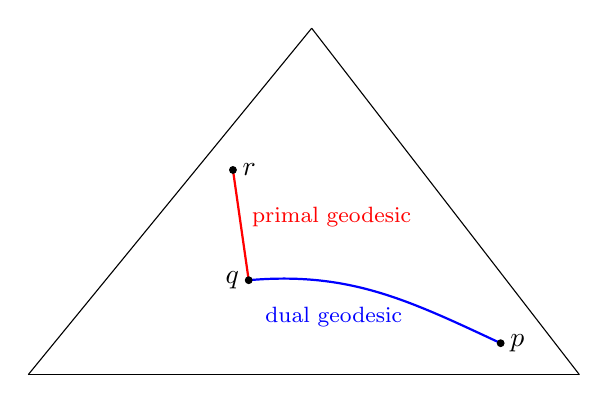
\begin{tikzpicture}[scale = 0.4]
%draw triangle
\draw (3.5, -2) to (-14, -2);
\draw (3.5, -2) to (-5, 9);
\draw (-14, -2) to (-5, 9);

%draw geodesics
\draw[thick, blue] (1, -1) to[out=155, in=5] (-7, 1);  % p to q
\draw[thick, red] (-7, 1) -- (-7.5, 4.5);  % q to r

\draw[black, fill] (1, -1) circle (3pt);
\node [right] at (1, -1) {$p$};
\draw[black, fill] (-7, 1) circle (3pt);
\node [left] at (-7, 1) {$q$};
\draw[black, fill] (-7.5, 4.5) circle (3pt);
\node [right] at (-7.5, 4.5) {$r$};

\node [blue, above] at (-4.3, -0.8) {{\footnotesize dual geodesic}};
\node [red, right] at (-7.2, 3) {{\footnotesize primal geodesic}};

\end{tikzpicture}
\caption{Generalized Pythagorean theorem for $L$-divergence.} \label{fig:pyth}
\end{figure}

\begin{theorem} [Generalized Pythagorean theorem] \label{thm:pyth}
Given $(p, q, r) \in \left(\Delta_n\right)^3$, consider the dual geodesic joining $q$ and $p$ and the primal geodesic joining $q$ and $r$. Consider the Riemannian angle between the geodesics at $q$. Then the difference
\begin{equation} \label{eqn:pyth}
{\bf D}\left[q \mid p\right] + {\bf D}\left[r \mid q\right] - {\bf D}\left[r \mid p\right]
\end{equation}
is positive, zero or negative depending on whether the angle is less than, equal to, or greater than $90$ degrees (see Figure \ref{fig:pyth}). 
\end{theorem}

Further properties of the Pythagorean theorem can be studied. To give a flavor we present an interesting result for the excess growth rate ${\bf T}_{\pi}\left[ \cdot \mid \cdot\right]$ defined by \eqref{eqn:excess.growth}.

\begin{figure}[t!]
\centering
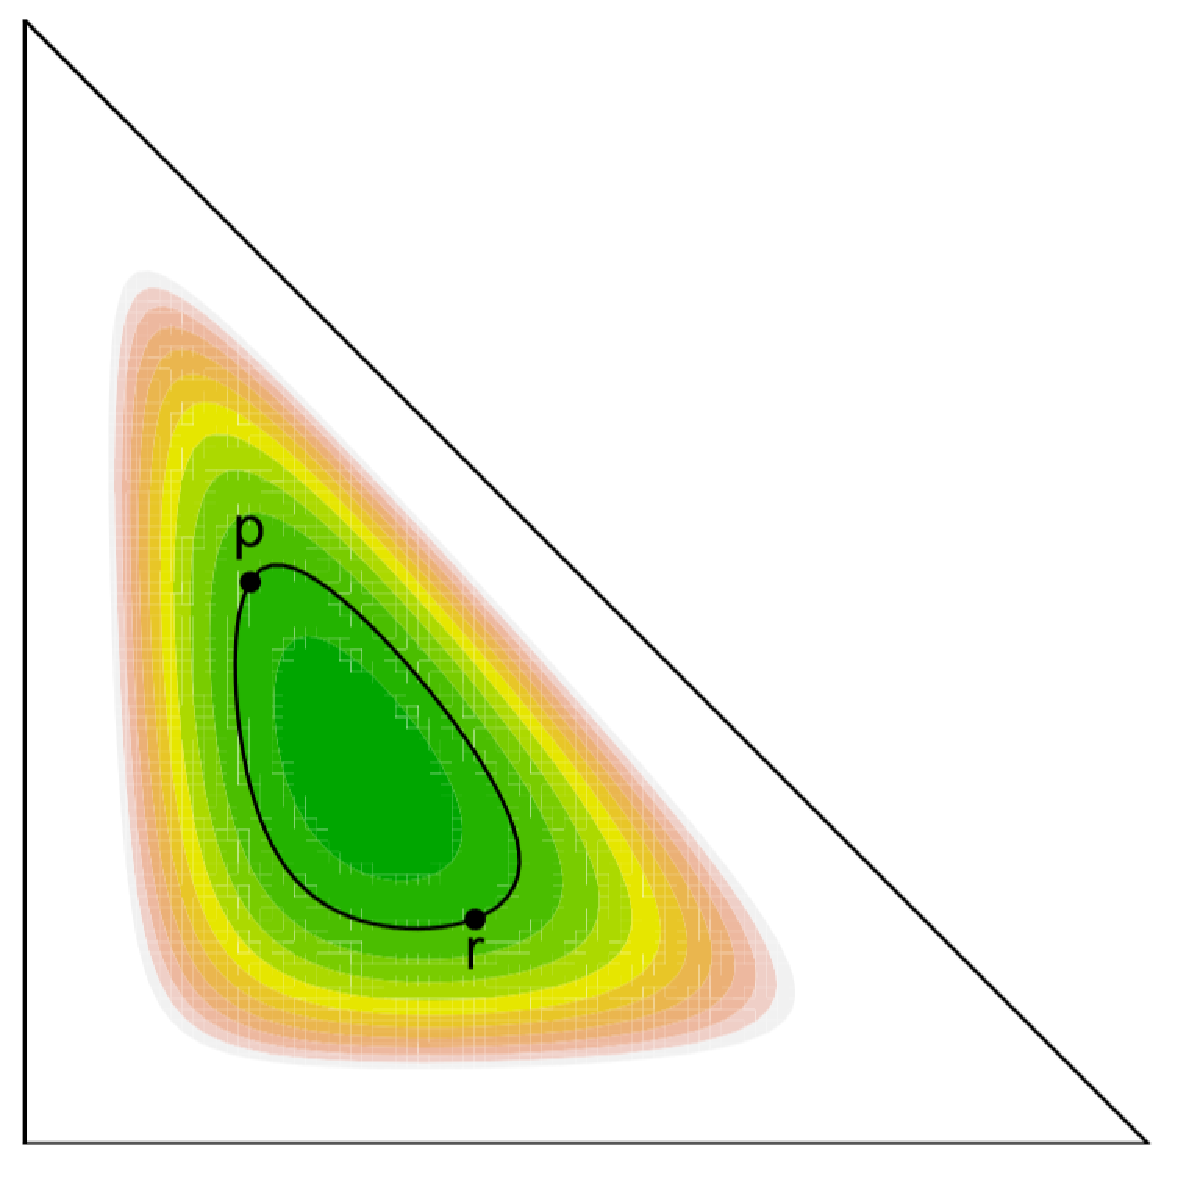
\includegraphics[scale=0.25]{pyth1.pdf}
\caption{The level sets of the map $q \mapsto {\bf T}_{\pi}\left[q \mid p\right] + {\bf T}_{\pi}\left[r \mid q\right] - {\bf T}_{\pi}\left[r \mid p\right]$ where $p$ and $r$ are fixed. Here $\pi = \overline{e}$ is the equal-weighted portfolio.} \label{fig:region}
\end{figure}


\begin{proposition}
Consider the excess growth rate ${\bf T}_{\pi}\left[ \cdot \mid \cdot\right]$ for a fixed portfolio weight vector $\pi \in \overline{\Delta}_n$. For $p, r \in \Delta_n$ fixed, the mapping
\begin{equation} \label{eqn:region}
q \in \Delta_n \mapsto f(q) := {\bf T}_{\pi}\left[q \mid p\right] + {\bf T}_{\pi}\left[r \mid q\right] - {\bf T}_{\pi}\left[r \mid p\right]
\end{equation}
is quasiconvex, i.e, the sublevel sets $\{q : f(q) \leq \lambda\}$ are convex (see Figure \ref{fig:region}). 
\end{proposition}
\begin{proof}
It suffices to show that the map
\[
g(x) := \log \left( \pi \cdot \frac{x}{p}\right) + \log \left( \pi \cdot \frac{r}{x}\right)
\]
is quasiconvex on $\Delta_n$. We will use the following characterization of quasiconvex functions (see \cite[Section 3.4.3]{BV04}): $g$ is quasiconvex if and only if
\begin{equation} \label{eqn:quasiconvex}
g(y) \leq g(x) \Rightarrow \nabla g(x) \cdot (y - x) \leq 0.
\end{equation}
for any $x$ and $y$.

Let $x, y \in \Delta_n$ be such that $g(y) \leq g(x)$. We have
\[
\partial_i g(x) = \frac{\frac{\pi_i}{p_i}}{\pi \cdot \frac{x}{p}} + \frac{-\frac{\pi_ir_i}{x_i^2}}{\pi \cdot \frac{r}{x}}.
\]
After some simplifications, we have
\begin{equation} \label{eqn:check.condition1}
\begin{split}
\nabla g(x) \cdot (y - x) &= \sum_{i = 1}^n \left(\frac{\frac{\pi_i}{p_i}}{\pi \cdot \frac{x}{p}} + \frac{-\frac{\pi_ir_i}{x_i^2}}{\pi \cdot \frac{r}{x}} \right) (y_i - x_i) \\
&= \frac{\pi \cdot \frac{y}{p}}{\pi \cdot \frac{x}{p}} - \frac{\sum_{i = 1}^n \pi_i \frac{r_i}{x_i} \frac{y_i}{x_i}}{\pi \cdot \frac{r}{x}}.
\end{split}
\end{equation}
Since $g(y) \leq g(x)$, we have
\[
\frac{\pi \cdot \frac{x}{p}}{\pi \cdot \frac{x}{p}} \leq \frac{\pi \cdot \frac{r}{x}}{\pi \cdot \frac{r}{y}}.
\]
Substituting this into \eqref{eqn:check.condition1}, we get
\begin{equation} \label{eqn:check.condition2}
\begin{split}
\nabla g(x) \cdot (y - x) &\leq \frac{\pi \cdot \frac{r}{x}}{\pi \cdot \frac{r}{y}} - \frac{\sum_{i = 1}^n \pi_i \frac{r_i}{x_i} \frac{y_i}{x_i}}{\pi \cdot \frac{r}{x}} \\
&= \frac{1}{\left(\pi \cdot \frac{r}{x}\right)\left(\pi \cdot \frac{r}{y}\right)} \left[ 
\left(\pi \cdot \frac{r}{x}\right)^2 - \sum_{i, j = 1}^n \pi_i \pi_j  r_ir_j \frac{1}{x_ix_j} \frac{y_j}{x_j} \frac{x_i}{y_i} \right] \\
&= \frac{1}{\left(\pi \cdot \frac{r}{x}\right)\left(\pi \cdot \frac{r}{y}\right)}  \sum_{i, j = 1}^n \frac{\pi_ir_i}{x_i} \frac{\pi_jr_j}{x_j} \left(1 - \frac{x_i}{y_i} \frac{y_j}{x_j} \right).
\end{split}
\end{equation}
Let $A = \sum_{i = 1}^n \frac{\pi_i r_i}{x_i}$ and let $\alpha_i = \frac{\pi_i r_i}{x_i}/A$. Note that $\alpha$ is a probability vector. Now we may write \eqref{eqn:check.condition2} in the form
\[
C \left(1 - \sum_{i, j = 1}^n \alpha_i \alpha_j \frac{x_i}{y_i} \frac{y_j}{x_j}\right),
\]
where $C > 0$ is a constant. Let $X$ and $Y$ be independent and identically distributed random variables such that
\[
{\Bbb P}\left(X = \frac{x_i}{y_i}\right) = {\Bbb P}\left(Y = \frac{x_i}{y_i}\right) = \alpha_i, \quad i = 1, \ldots, n.
\]
By Jensen's inequality, we have
\[
\sum_{i, j = 1}^n \alpha_i \alpha_j \frac{x_i}{y_i} \frac{y_j}{x_j} = {\Bbb E} \left[ X \cdot \frac{1}{Y}\right] = {\Bbb E} [X] {\Bbb E} \left[\frac{1}{Y}\right] \geq {\Bbb E}[X] \frac{1}{{\Bbb E}[X]} = 1.
\]
Thus $\nabla g({\bf x}) \cdot (y - x) \leq 0$ and we have proved that $g$ is quasiconvex.
\end{proof}

\subsection{Optimal rebalancing frequency}
Finally we mention a practical problem related to the $L$-divergence. The generalized Pythagorean theorem gives a geometric way to study the rebalancing frequency of a functionally generated portfolio. To give a simple example, consider the empirical example as in Figure \ref{fig:simplex} and the equal-weighted portfolio $\boldsymbol{\pi}(p) \equiv \overline{e} = \left(\frac{1}{3}, \frac{1}{3}, \frac{1}{3}\right)$.

\begin{figure}[t!]
\centering
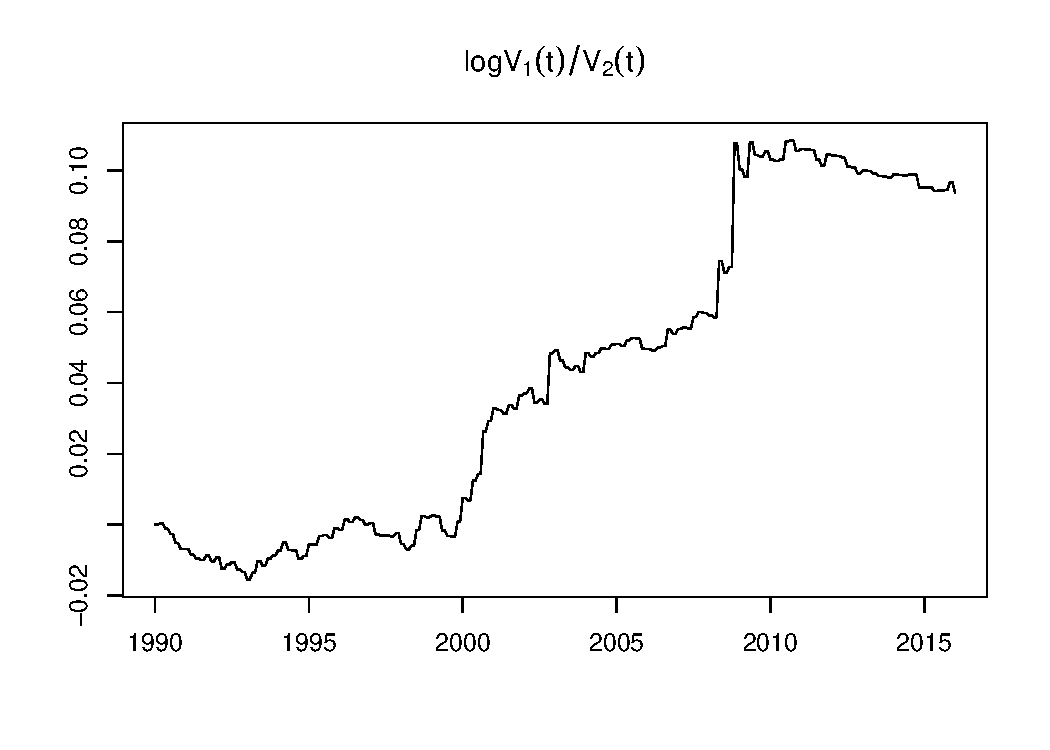
\includegraphics[scale=0.42]{example1.pdf}
\caption{Relative performance of the portfolio $V_1$ (rebalanced every month) versus $V_2$ (rebalanced every two months).} \label{fig:example1}
\end{figure}

Consider two ways of implementing this portfolio: (i) rebalance every month; (ii) rebalance every two months. If $V_1$ and $V_2$ denote respectively the values of these implementations, Figure \ref{fig:example1} plots the time series of the relative performance $\log V_1(t) / V_2(t)$. For this data set, rebalancing every month boost the return by about $10\%$ in log scale. Using the decomposition \eqref{eqn:multiplicative.decomp}, we see that if $T$ is the terminal time, then
\begin{equation*}
\begin{split}
& \log \frac{V_1(T)}{V_2(T)}\\
&= \sum_k \left({\bf D}\left[\mu(2k + 1) \mid \mu(2k) \right] + {\bf D}\left[\mu(2k + 1) \mid \mu(2k + 2)\right] - {\bf D}\left[\mu(2k + 2) \mid \mu(k)\right]  \right).
\end{split}
\end{equation*}
By Theorem \ref{thm:pyth}, the sign of each term is determined by the Riemannian angle of the geodesic triangle. This angle summarizes in a single number the correlation among the stock returns that is relevant to the rebalancing frequency. Further work should study the joint relationship between the angle and the {\it size} of the geodesic triangle which determines the magnitude of \eqref{eqn:pyth}.


\begin{figure}[t!]
\centering
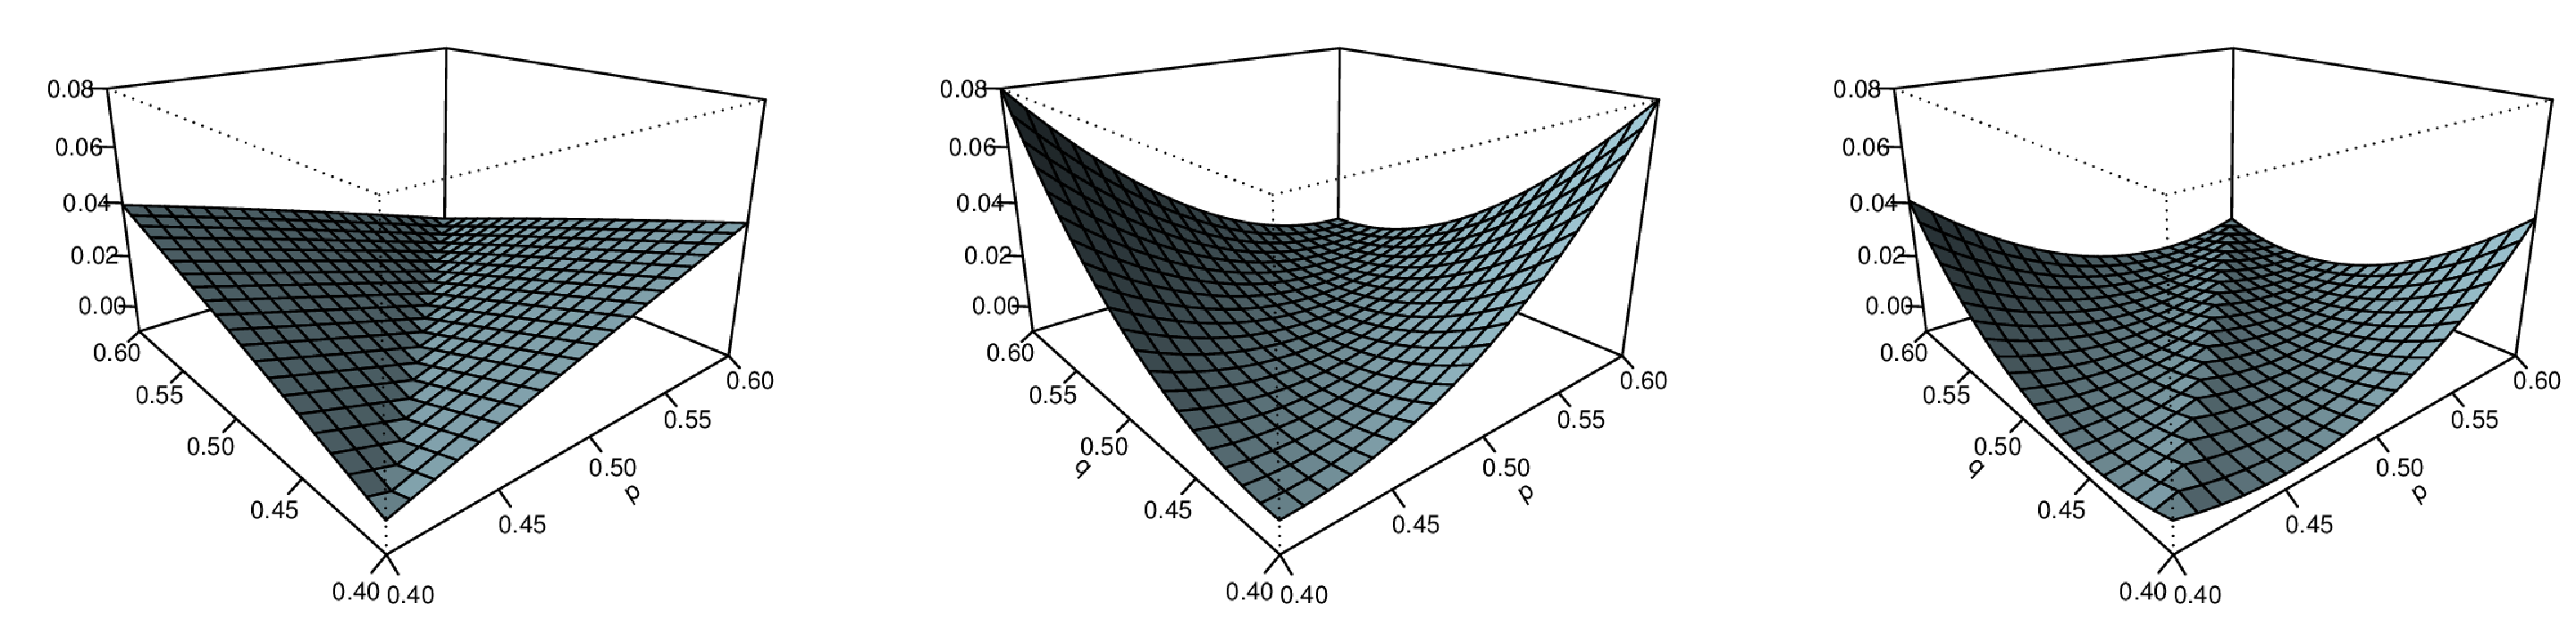
\includegraphics[scale=0.22]{divergence2.pdf}

\caption{Left: Transaction cost ${\bf C}\left[q \mid p\right]$. Middle: The $L$-divergence ${\bf D}\left[q \mid p\right]$. Right: The difference ${\bf D} - {\bf C}$. In these figures $n = 2$ and the $x$ and $y$-axes are the first coordinates of $p$ and $q$ respectively.} \label{fig:example1}
\end{figure}

In practice trading incurs transaction costs which have been neglected so far. Transaction costs create a drag of the portfolio value. A common setting is that the transaction cost is {\it proportional}, i.e., we pay a fixed percentage of the value exchanged. In our model, the transaction cost may be approximated by a functional ${\bf C}\left[q \mid p\right] \geq 0$ where $p$ and $q$ are the beginning and ending market weights of the holding period (Figure \ref{fig:example1}). Since the transaction cost is proportional, the cost is of linear order when $q \approx p$. On the other hand, the $L$-divergence is approximately quadratic when $q \approx p$.  Thus the net difference ${\bf D}\left[q \mid p\right] - {\bf C}\left[ q \mid p \right]$ is negative when $q$ is sufficiently close to $p$. Financially, this means that the investor should not rebalance too often -- at least when the increments of the market weights are `small'. We end this paper with the following problem:

\begin{problem}
Design a robust strategy for rebalancing a given trading strategy.
\end{problem}

%\begin{acknowledgement}
%\end{acknowledgement}
%
%\section*{Appendix}
%\addcontentsline{toc}{section}{Appendix}

\bibliographystyle{abbrv}
\bibliography{geometry.ref}


\end{document}
